\chapter{腹膜腔与腹壁}

\section{检查方法}

\subsection{扫描前准备}

一般无需做特殊准备,常在扫描前空腹4~6小时,扫描前1~2小时口服1.5%~2%复方泛影葡胺400~600ml,在患者上床前15分钟再口服300ml。如检查腹壁则不一定常规口服造影剂。

\subsection{扫描方法}

其扫描方法与腹腔内实质性器官基本相同。①患者一般采取仰卧位扫描,为了将腹膜腔病灶与肠管等结构分开,可灵活采取俯卧位或左、右侧卧位。②扫描范围一般应将胸腔下部包括在内,以便于区分胸腔积液与腹腔积液、网膜囊上隐窝积液与膈下其他间隙积液。③为了显示肠系膜血管和水肿、腹膜肿瘤和炎症,宜作增强扫描。一般以2~3ml/s流率静注有机碘剂100ml。择情行动脉期、门静脉期和平衡期扫描。④为了显示系膜、韧带,需要选择恰当的窗技术参数,窗宽宜宽些、窗位宜低些,这样它所显示的图像层次和内容物将比较丰富。⑤为了更准确、直观的作出解剖定位诊断,可作其他方位(如矢状、冠状)或三维立体图像重建。

\section{正常解剖}

\subsection{腹膜腔和腹腔的概念}

1.腹膜:属浆膜组织,由单层间皮细胞和含弹性纤维的结缔组织所组成。其总面积几乎和皮肤的面积相等。根据其位置分布分为两类:①壁层腹膜:即衬覆于腹壁、盆腔内表面的腹膜;②脏层腹膜:即覆盖于腹腔、盆腔脏器表面的腹膜。壁层腹膜较厚;而脏层腹膜呈半透明状与脏器紧密相连不易剥离,因此无论从形态、机能和临床病理角度往往将脏层腹膜当作该脏器的组成部分。

腹膜从腹、盆壁移行于器官,或由一个器官移行到另一个器官,其移行的部分常形成许多网膜结构,包括网膜系膜、韧带和皱襞,对器官起支持、固定作用。

2.腹膜腔:脏、壁两层腹膜在后腹壁互相融合形成一个潜在的腔隙即腹膜腔。其形态不规则,内有70~80ml浆液。男性腹膜腔是完全闭合的;女性借输卵管伞端、子宫腔和阴道与体外构成潜在性通道。腹膜腔又可分成大小两部分:①小腹膜腔:亦称小网膜囊,位于小网膜和胃后方;②大腹膜腔:则为小网膜囊以外的腔隙。大小腹膜腔借网膜孔相通,两者的关系犹如大房中的小房(图\ref{fig18-1})。

\begin{figure}[!htbp]
 \centering
 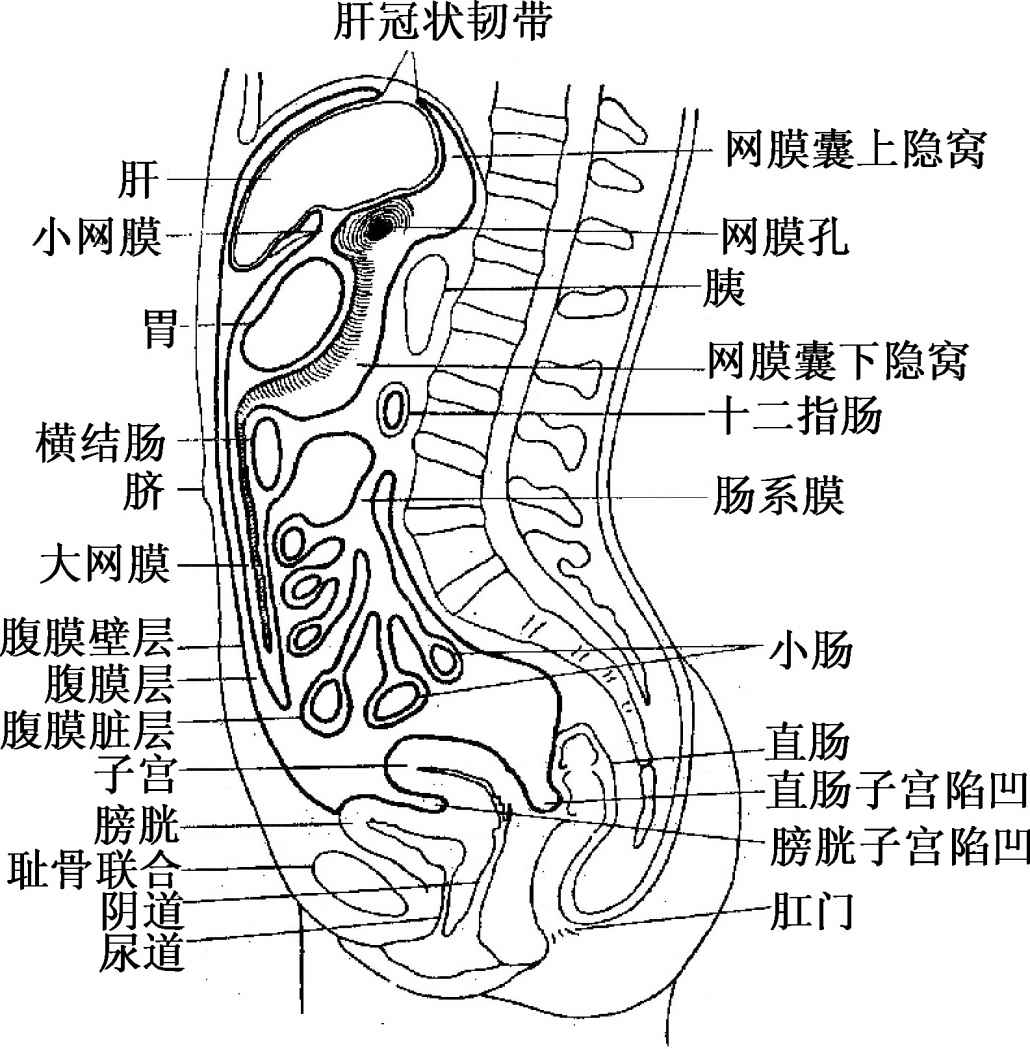
\includegraphics[width=.7\textwidth,height=\textheight,keepaspectratio]{./images/Image00370.jpg}
 \captionsetup{justification=centering}
 \caption{腹膜(正中切面,女,左侧观)}
 \label{fig18-1}
  \end{figure} 

3.腹腔:是指小骨盆上口以上、由腹壁围成的腔,广义的腹腔还包括盆腔在内。它与腹膜腔从解剖学意义上讲是有区别的,腹腔包括腹膜腔和腹膜后腔,腹膜腔是腹腔的一部分。腹腔内所有脏器位于腹膜腔之外。

\subsection{间位和外位器官}

1.腹膜内位器官:即器官表面几乎全部被腹膜包裹者,如胃、十二指肠上部、空肠、回肠、盲肠、阑尾、横结肠、乙状结肠、直肠上段、脾、胰尾、卵巢及输卵管等。

2.腹膜间位器官:即器官3面或绝大部分被覆有腹膜者,如升结肠、降结肠、直肠中段、肝、胆囊、膀胱及子宫等。

3.腹膜外位器官:亦名腹膜后位器官。即器官仅一面覆盖有腹膜。这些器官多位于腹膜之后,与腹后壁相贴附,如十二指肠降部和下部、直肠下段、胰腺头颈体部、肾上腺、肾及输尿管等。

\subsection{大网膜和小网膜}

1.大网膜:连于胃大弯与横结肠之间,似围裙状垂于小肠和结肠前方。大网膜由4层腹膜构成。前两层是由胃前后壁的脏腹膜自胃大弯下垂而成,当下垂至腹下部后折转向上形成后两层、向上包裹横结肠,移行为横结肠系膜,并与腹后壁腹膜相延续。在成人4层常在横结肠平面愈合在一起,而从胃大弯到横结肠的前两层网膜称为胃结肠韧带。

2.小网膜:是连于肝门与胃小弯及十二指肠上部之间的双层腹膜,自肝静脉韧带裂发出,向下、左展开。其中肝门与胃小弯之间的部分称肝胃韧带,肝门与十二指肠上部之间的部分称肝十二指肠韧带。后者的右缘游离,其内含有胆总管、肝固有动脉和门静脉等,肝十二指肠韧带的后方是网膜孔。

\subsection{网膜囊}

网膜囊壁的组成:①前壁是小网膜、胃后壁、大网膜的前两层;②后壁是大网膜的后两层、横结肠及其系膜和覆于胰、左肾、左肾上腺的腹膜;③上壁是肝尾状叶与膈下面的腹膜,上方在右侧由尾状叶向右、上方突入上隐窝内,由于腹膜反褶使肝尾叶的后、左、前、下诸方均有潜在间隙;④下壁是大网膜第二、第三层的愈着部;⑤左壁是脾胃韧带、脾和脾肾韧带;⑥右侧上份为下腔静脉、下份为肝十二指肠韧带及十二指肠上部。

网膜囊分为上、下两部分。①上部分包括上隐窝、前庭及网膜孔。上部分较小,居中线区域后份,主要与肝尾状叶相邻。上部分前壁即小网膜,它有效的将左肝上后间隙与网膜囊上隐窝分开。②下部分包括下隐窝及左侧向上方突出的脾隐窝。下部分显著大于上部分,居中线及左上腹后份,主要与胃后壁(下隐窝前方为胃后壁)、胰腺及左肾上腺相邻。

上下两部分之间即胃胰裂,它与前方的胃小弯及所组成的孔道是网膜囊上下两部分之间的分界线和通道。在胃胰裂下方,还可能存在腹膜反折所形成的皱襞,是一种并非少见的解剖变异,它对于炎症或积液在上、下两部分之间的扩散有一定限制作用。

\subsection{胃胰襞}

腹腔动脉于T\textsubscript{12} ~L\textsubscript{1}
平面由腹主动脉发出,向前行一定距离(一般约2.5cm)即分出肝总动脉和胃左动脉,并将后腹膜向前掀起形成胃胰襞,且形成一弧形的游离缘,与其前方的胃小弯形成一孔道,成为网膜囊上、下两部分的分界线,此孔道大小有一定变异。在孔道稍下方可能出现上述的腹膜反褶变异所形成的隔膜。

\subsection{肠系膜}

系膜主要指将肠管连至腹后壁的双层腹膜结构。两层间夹有血管、神经、淋巴管、淋巴结和脂肪等。

1.小肠系膜:呈折扇形将空、回肠连于腹后壁,其附于腹后壁的部分称小肠系膜根。它从第2腰椎左侧斜向右下方,止于右骶髂关节前方,长约15cm。其右侧方为右结肠下间隙,左侧方为左结肠下间隙,前者相对比较封闭,后者下方与盆腔间是开放的。

2.阑尾系膜:将阑尾连于小肠系膜下端,呈三角形。

3.横结肠系膜:连于横结肠与腹后壁之间,其根部起自结肠右曲,向左跨右肾中部、十二指肠降部、胰腺前缘、左肾中部,止于结肠左曲。

4.乙状结肠系膜:将乙状结肠连于盆壁之间,其根部附着于左髂窝和骨盆右后壁。

\subsection{韧带及相应的间隙或隐窝}

韧带是连于腹壁与器官,或连于相邻器官之间的腹膜结构。对器官有固定或悬吊作用。①肝的韧带:除前述的肝胃韧带、肝十二指肠韧带外,还有镰状韧带、冠状韧带和左、右三角韧带及肝肾韧带等。②脾的韧带:主要有胃脾韧带和脾肾韧带。

\subsubsection{镰状韧带}

位于肝脏前方、居中线右侧,由上向下纵行,为左右肝上间隙的分界线。它是腹前壁上部与肝上面之间的双层腹膜结构,呈矢状位,其游离缘内含有肝圆韧带。上方左侧与肝左三角韧带前层相延续,右侧与冠状韧带上层相延续。镰状韧带并非肝左、右叶的分界。

\subsubsection{冠状韧带、肝右三角韧带、肝肾韧带及右侧肝周间隙}

1.对冠状韧带的位置过去存在着许多错误认识。现证明:①冠状韧带位于肝脏右叶后段与膈肌后部之间,而且冠状韧带分为上、下两层;②两层在外侧融合为肝右三角韧带;③腹膜在冠状韧带下层外分,向下、内反褶形成肝肾韧带。肝肾韧带居右肝下间隙,附着于肝右叶脏面与右肾上、前面之间,它对右肝下间隙积液或脓肿有一定分隔作用。

2.由于冠状韧带在肝后部的分隔,故右侧肝周区域存在着3个间隙:①右肝上间隙,位于真正的右膈下;②右肝下间隙;③肝裸区:位于冠状韧带上、下层之间,属腹膜后间隙的一部分。近年的研究证明肝裸区与右肾周间隙之间可能相互通连。

3.肝肾隐窝的毗邻关系:肝肾隐窝是右肝下间隙的后上部分,也是腹膜腔最靠后的部分。它的毗邻关系如下:①上方以冠状韧带下层为界;②下方为结肠肝曲或横结肠系膜起始部;③内侧上部分为网膜孔并与网膜囊相通,内侧下部分为十二指肠降部;④外侧与结肠旁沟和右肝上间隙相通;⑤前方为肝脏脏面的右肾压迹区域;⑥后方为右肾上极。

由于肝肾隐窝在仰卧位时位置最低,因此是炎症、外伤、积液等腹腔内液体首先积聚的部位。

\subsubsection{肝左三角韧带及左侧肝周间隙}

1.肝左三角韧带:对其位置、长度过去亦存在着很大争议。国内闵鹏秋等研究证明:左三角韧带均由内向外行走于膈与肝左叶之间,82.5%超过肝左叶外缘后,仍继续向外并附着于左膈下,形成一游离段,这样位于肝上方的左三角韧带就有效地将肝左上区域分隔成上前、上后两个间隙。但两间隙下方均可分别与肝胃隐窝相通连。

2.从上述可知左肝周包括3个间隙:①上前间隙;②上后间隙;③肝胃隐窝:位居肝脏面与横结肠及其系膜之间,后方以小网膜(肝胃韧带)与网膜囊分开。

\subsubsection{肝胃韧带}

即小网膜的主要组成部分。向外上后延伸,在矢状中线附近,向上先附着于左膈,然后再折向前与肝左三角韧带后层相续。因此,肝胃韧带将左肝上后间隙与网膜囊上隐窝分开。

\subsubsection{胃脾韧带及脾肾韧带}

1.胃脾韧带:从胃大弯连接脾蒂,此韧带的前方为胃脾隐窝。

2.脾肾韧带:从左肾外前缘向外连接脾蒂,此韧带的后方为脾肾隐窝。

胃脾韧带和脾肾韧带之间即网膜囊下隐窝外侧份。

\subsubsection{膈结肠韧带、胃结肠韧带}

1.膈结肠韧带:附着于左膈外份与结肠脾曲之间、脾下极下方,由后向前形成一游离缘。它在一定程度上限制着左膈下方与左结肠旁沟之间液体的相互对流。

2.胃结肠韧带:从胃大弯侧到横结肠的两层网膜称为胃结肠韧带。

\subsubsection{结肠下间隙和结肠旁沟}

1.结肠下间隙:从盲肠至乙状结肠形成了一个结肠框,此框范围内即为结肠下间隙。由于小肠系膜根部由左上斜向右下而将其进一步分为两部分:①右结肠下间隙:上为横结肠右半及其系膜,外侧为升结肠,下内方为小肠系膜,近似一封闭的三角形。②左结肠下间隙:上为横结肠左半及其系膜,外侧为降结肠,内侧为小肠系膜,下方与盆腔相通连。

2.结肠旁沟:在升、降结肠与侧腹壁之间,即为右结肠旁沟和左结肠旁沟。

\subsection{盆腔的陷凹(隐窝)}

1.膀胱直肠陷凹、膀胱子宫陷凹、直肠子宫陷凹:腹膜沿膀胱后壁向下至盆底,然后反褶向上,男性附着于直肠前壁,形成直肠膀胱陷凹;女性则先被覆于子宫形成膀胱子宫陷凹,然后再折向后下附着于直肠形成直肠子宫陷凹。正常情况下很少有积液。

2.直肠周围陷凹:即在直肠膀胱陷凹两侧,向直肠旁呈弧形走行的较小隐窝。

3.膀胱旁(盆外侧)陷凹:此隐窝位于直肠膀胱陷凹两侧稍上,它们从左右两侧分别与结肠旁沟相延续,是左右结肠旁沟与直肠膀胱陷凹间的通道。

\subsection{腹膜腔的解剖划分}

腹膜腔由脏器、韧带、系膜分隔成许多潜在的间隙、隐窝、陷凹。国内作如下解剖划分:

1.上腹腔:

右侧:肝上间隙、肝下间隙、肝裸区(应属腹膜后间隙)。

左侧:肝上前间隙、肝上后间隙、肝胃隐窝、胃脾隐窝、脾肾隐窝、脾外侧间隙、网膜囊(上、下两部分)。

2.下腹腔:

右侧:右结肠下间隙、右结肠旁沟。

左侧:左结肠下间隙、左结肠旁沟。

3.盆腔:

膀胱直肠隐窝(女性为膀胱子宫隐窝及子宫直肠隐窝)、膀胱旁(盆外侧)隐窝、直肠周围隐窝。

\subsection{腹壁}

腹壁以腋后线为界分为前外侧壁和后外侧壁。前外侧壁的上界为胸骨剑突、肋弓及第11、第12肋的游离缘;下界为耻骨联合、腹股沟及髂嵴。该区域的腹壁厚度因人而异,由浅入深腹壁有6层:即皮肤、皮下组织(或称浅筋膜)、肌层、腹横筋膜、腹膜外脂肪层及壁层腹膜。其中肌层包括腹直肌、腹外斜肌、腹内斜肌和腹横机。

中部和下部腰椎水平层面CT可清晰显示上述诸肌。在脐部无脂肪组织,皮肤、筋膜和腹膜直接相连。半月线又称Spigelian筋膜,由3条前外侧肌的腱膜在腹直肌外缘连合而成。扫描层在坐骨孔水平时可见腹直肌占据大部分前腹壁。脐旁筋膜位于脐的下部,环绕脐尿管。在膀胱区可将腹膜外脂肪分为位于脐旁筋膜前的膀胱前间隙和位于脐旁筋膜后的膀胱周围间隙。

\section{腹腔积液、脓肿、炎症和网膜缺血}

\subsection{腹腔积液}

腹腔积液系指腹膜腔内游离液体的异常积聚。积聚于腹膜腔内的液体临床上常称为腹水。它仅是一种病症,不是一个独立的疾病。

\textbf{【病因】}
全身性和(或)局部的原因均可导致液体从血管和淋巴管渗出或漏出到腹膜腔。①全身因素:常见于低蛋白血症、钠水潴留、内分泌障碍。②局部因素:常见于肝硬化门脉高压、腹膜炎、腹膜恶性肿瘤或恶性肿瘤腹膜种植,以及胸导管或乳糜池的阻塞。

\textbf{【分类】}
①按其性质分为:渗出液和漏出液;②按其成分可分为:浆液性、黏液性、血性、脓性、乳糜性、胆汁性、尿液和脑脊液性等。

\textbf{【临床表现】}
单纯就腹水而言,少量腹水可以无明显症状,中量以上腹水时出现腹围增大,腹内压增高,有时可见脐疝形成,横膈抬高产生呼吸困难和心悸。依病因不同还有相应的症状如发热、腹痛、腹部包块、肝大、水肿等。

\textbf{【CT表现】}

1.常见表现:①腹水最早的征象是腹膜反折处因液体积聚而增厚,最常见于肾前筋膜和侧锥筋膜。②结肠上区的积液开始于右肝下间隙和肝肾隐窝内,尔后溢入右膈下,表现为肝腹侧及外侧缘新月形低密度影。③结肠下区少量腹水易停留在盆腔的陷凹内。左侧结肠下区的液体流入盆腔时,常在乙状结肠系膜前停滞;而右侧结肠下区的液体从小肠系膜隐窝向回盲瓣区流动,由于腹水的衬托可见小肠系膜叶。进入盆腔的液体,病人体位变更时又可经结肠旁沟向头端流入右肝下和(或)右膈下间隙。④大量腹水时可见腹腔内脏器的周围均匀一致的低密度带,从而使脏器向心性集中(图\ref{fig18-2})。充盈对比剂的小肠曲呈漂浮状或有下沉样表现。当腹水进一步增多时可形成“张力”性腹水,可见肠管向一侧推移,受压的血管和系膜呈薄线状;有的类似占位性病变;有时并发腹疝。部分可显示腹水的病因如肿瘤、炎症等。

\begin{figure}[!htbp]
 \centering
 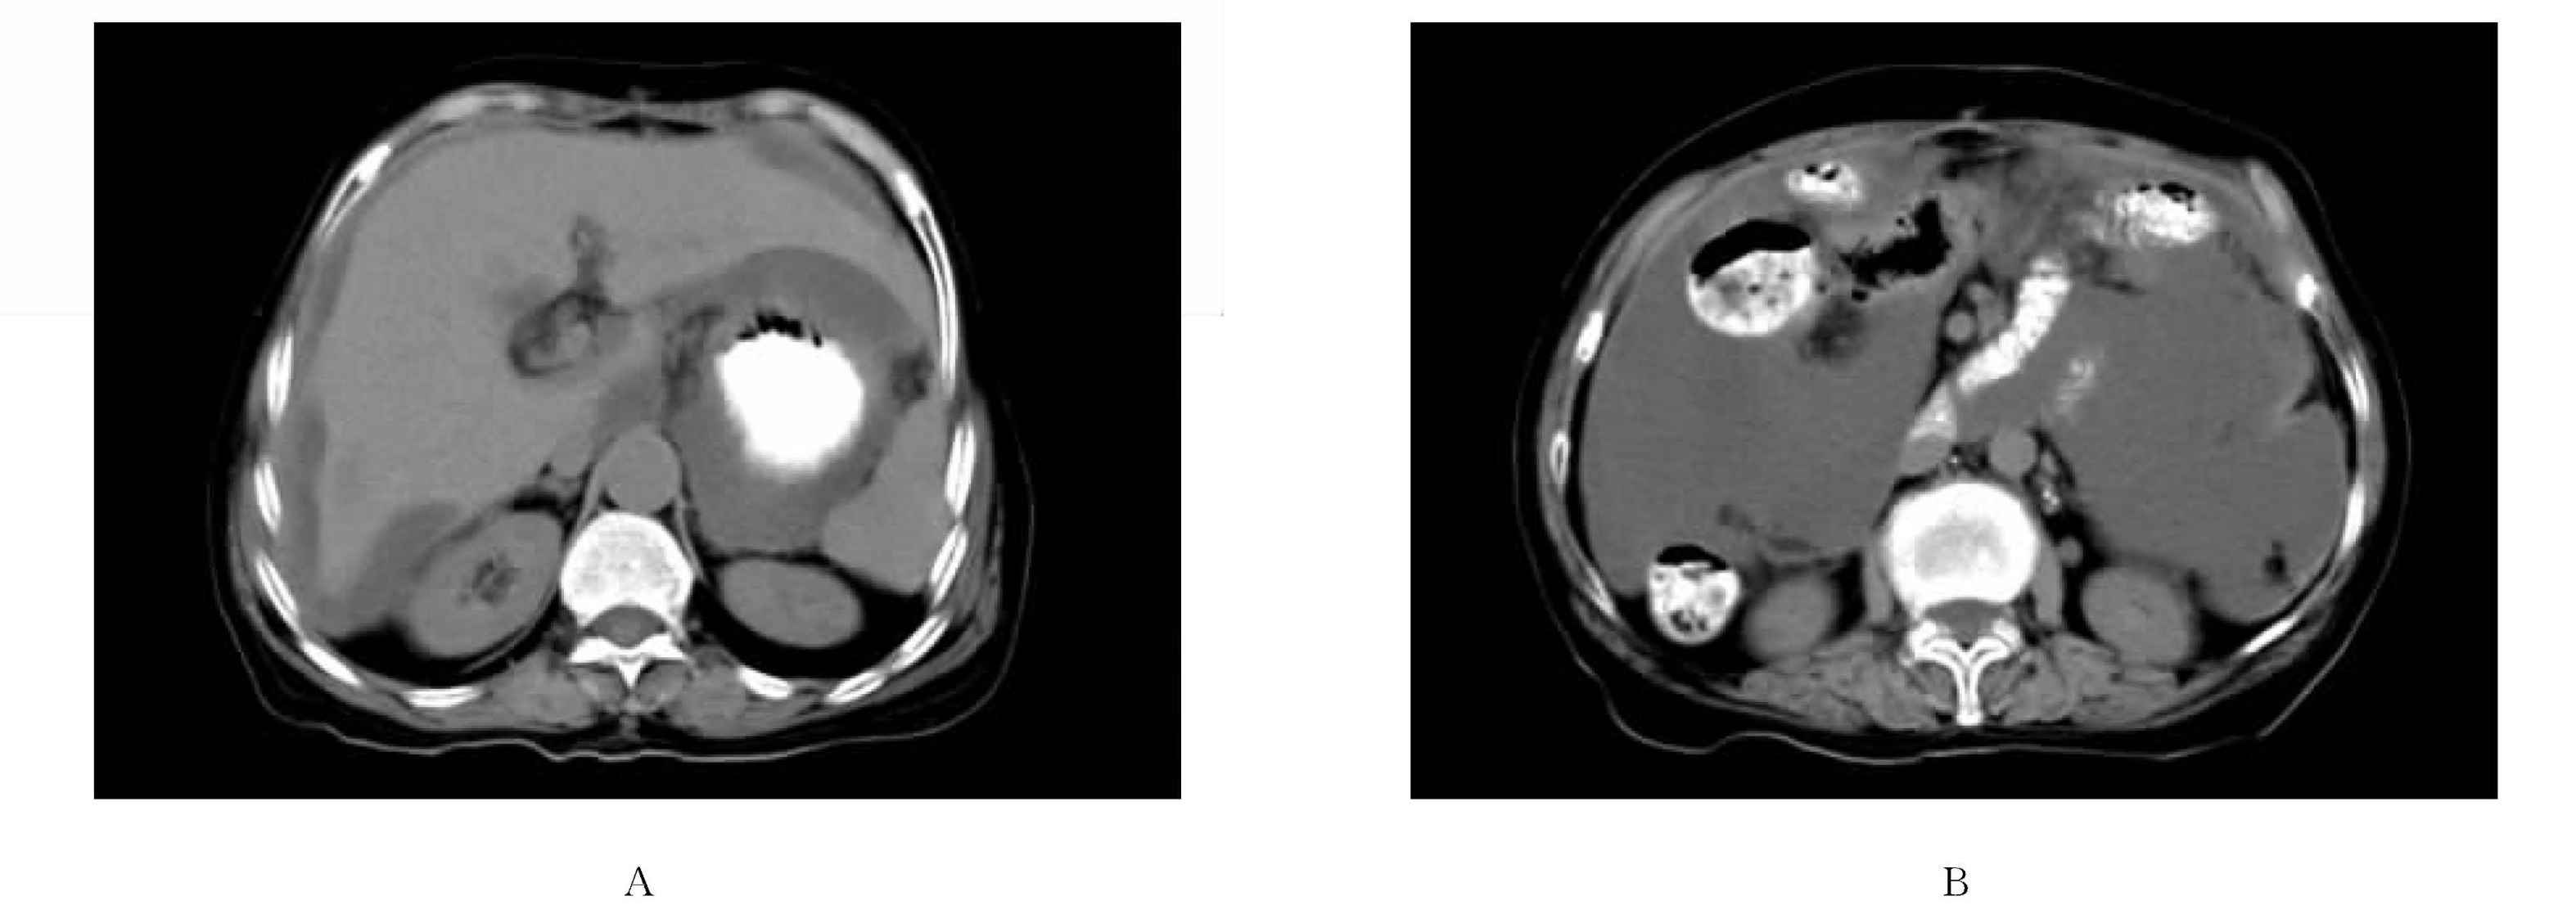
\includegraphics[width=.7\textwidth,height=\textheight,keepaspectratio]{./images/Image00371.jpg}
 \captionsetup{justification=centering}
 \caption{腹水\\{\small A、B为同一患者,肝、脾、胃肠周围有大量水样密度区,小肠曲呈漂浮状}}
 \label{fig18-2}
  \end{figure} 

2.腹腔积液的CT值高低与蛋白含量有关,利用CT值测量可以大体区分腹腔积液的成分:①乳糜液:一般CT值为负值;②漏出液:CT值较低,一般<18Hu;③渗出液:CT值较高,>18Hu;④血性液:更高些,可>30Hu。而且国内外学者多以20Hu为高、低密度腹水的界值,即>20Hu者为高密度腹水。

3.腹水量的估计:①大量:腹水充满腹腔和盆腔。②中量:限于肝脾周围。③少量:仅限于结肠旁沟等处。

\subsection{腹腔积气}

腹腔积气习惯称为气腹。

\textbf{【病因】}
胃肠道内气体、外界气体或产气杆菌感染引起的腹膜炎均可使气体游离于腹腔内产生气腹,以胃肠道穿孔最多见。此外,见于人工气腹、腹部手术后(正常情况下,术后7~10天气体吸收干净)、腹腔穿刺及腹腔镜检查后、输卵管通气、子宫输卵管破裂(自发、医源如剖宫产等)、肠壁气囊肿破裂等。间质性肺炎伴间质性肺气肿或纵隔积气时,气体可经血管周围间隙弥散入腹腔。故气腹并非一定是胃肠道穿孔,而且胃肠道穿孔过小或穿孔口被食物、血块所堵塞等原因亦可无气腹出现。

\textbf{【临床表现】}
腹腔积气除剖腹术后正常的气体残留、肠气囊肿破裂,以及诊断性人工气腹等,一般多合并有腹膜炎和腹腔脓肿,故常合并不同程度的腹膜腔感染的症状、体征和化验异常。

\textbf{【CT表现】}
气体可以是大量的,也可以少量的,甚至仅见少许小气泡。由于气体的衬托可以显示出腹腔内的脏壁层腹膜、韧带、粘连带等。在CT扫描时应注意窗技术的应用,窗宽太窄气体不易与脂肪相区别(图\ref{fig18-3})。

\begin{figure}[!htbp]
 \centering
 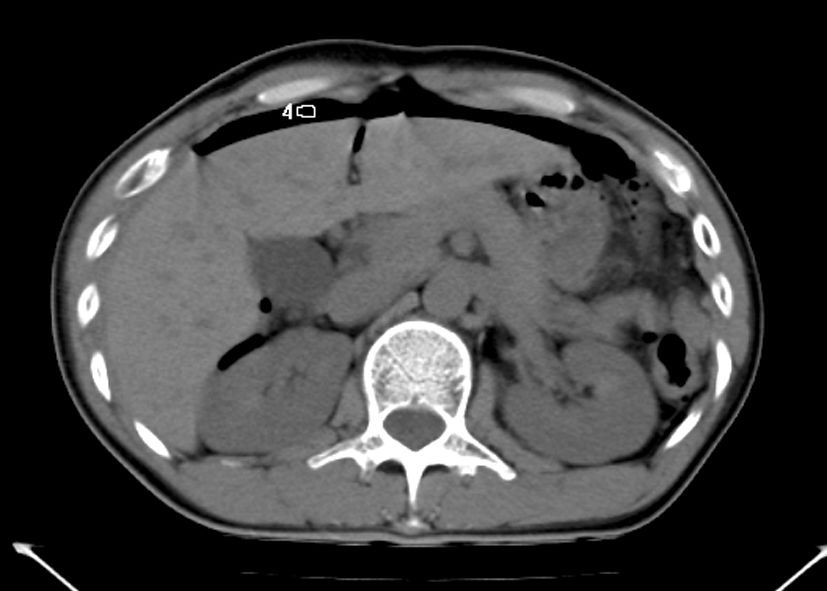
\includegraphics[width=.7\textwidth,height=\textheight,keepaspectratio]{./images/Image00372.jpg}
 \captionsetup{justification=centering}
 \caption{气腹\\{\small 前腹壁下、肝下间隙有低密度积气}}
 \label{fig18-3}
  \end{figure} 

\subsection{腹腔脓肿}

\textbf{【病因病理】}
腹腔脓肿通常是腹膜炎的局限化,系指腹腔内某一间隙或部位的局部脓肿,内含脓液、坏死组织、细菌和白细胞,常由腹腔内肠曲、内脏、腹壁、网膜或系膜等包裹粘连而成。按其发生部位主要有以下几类:

1.膈下脓肿:是指横膈以下、横结肠及系膜以上区域的局限性脓肿,包括右肝上、右肝下、左肝上前、左肝上后间隙脓肿和网膜囊脓肿。有原发和继发之分。原发者少见,其发病原因尚不明确。后者常继发于腹部感染灶,约占85%,其中60%继发于急性阑尾炎穿孔、胃及十二指肠溃疡穿孔、肝胆系统疾病;相对少见的有腹部创伤、腹膜后区感染或胸腔化脓性疾病的扩散。

2.盆腔脓肿:一般先发生在膀胱直肠隐窝(女性则为膀胱子宫隐窝及子宫直肠隐窝),然后扩散到两侧盆腔的侧隐窝。病因大致与膈下脓肿相仿,但常是腹壁尤其盆腔术后、阑尾炎、盆腔炎等所致。

3.肠曲或系膜间脓肿:也称为下腹腔脓肿,是指横结肠系膜以下、盆腔以上区域的局限性脓肿。脓肿位于肠曲或肠系膜之间,占腹腔脓肿的4%。可分为右结肠下间隙脓肿、左结肠下间隙脓肿、右结肠旁沟脓肿、左结肠旁沟脓肿。病因可以是膈下或盆腔脓液流注肠间,亦可为肠管、肠系膜局部外伤、炎症等所致。

腹腔脓肿以膈下和盆腔脓肿最常见,膈下脓肿较复杂。膈下脓肿大多位于右肝下间隙。

\textbf{【临床表现】}
一般均有腹痛及感染所致的全身反应,如寒颤、发热、心率快,白细胞增多及核左移等。经抗炎治疗后上述症状消失,一旦停药后其异常症状可再度出现。此外,还可有局部的压痛、反跳痛、叩击痛等。

\textbf{【CT表现】}
腹膜腔脓肿一般均受腹膜腔间隙、隐窝所限,并以脏器、韧带、系膜等作其周壁。脓肿早期为软组织密度样肿块;增强扫描无明显强化。脓肿坏死液化后结缔组织包绕,中央近水样低密度,而周边密度稍高(图\ref{fig18-4});增强扫描呈环形强化。邻近脏器和组织结构受压移位。胸腔可见反应性胸水;膈下脓肿可破入胸腔出现脓胸、肺脓肿或支气管胸膜瘘。脓腔25%~50%出现低密度气体影,甚至出现液气平面。可以是产气菌感染所致,亦可是脓肿与肠道交通的结果。气泡的出现不是特征性,但可高度提示诊断。类似的表现亦可见于肿瘤坏死或囊肿继发感染或与肠道沟通时,肿块内偶见气体。

\begin{figure}[!htbp]
 \centering
 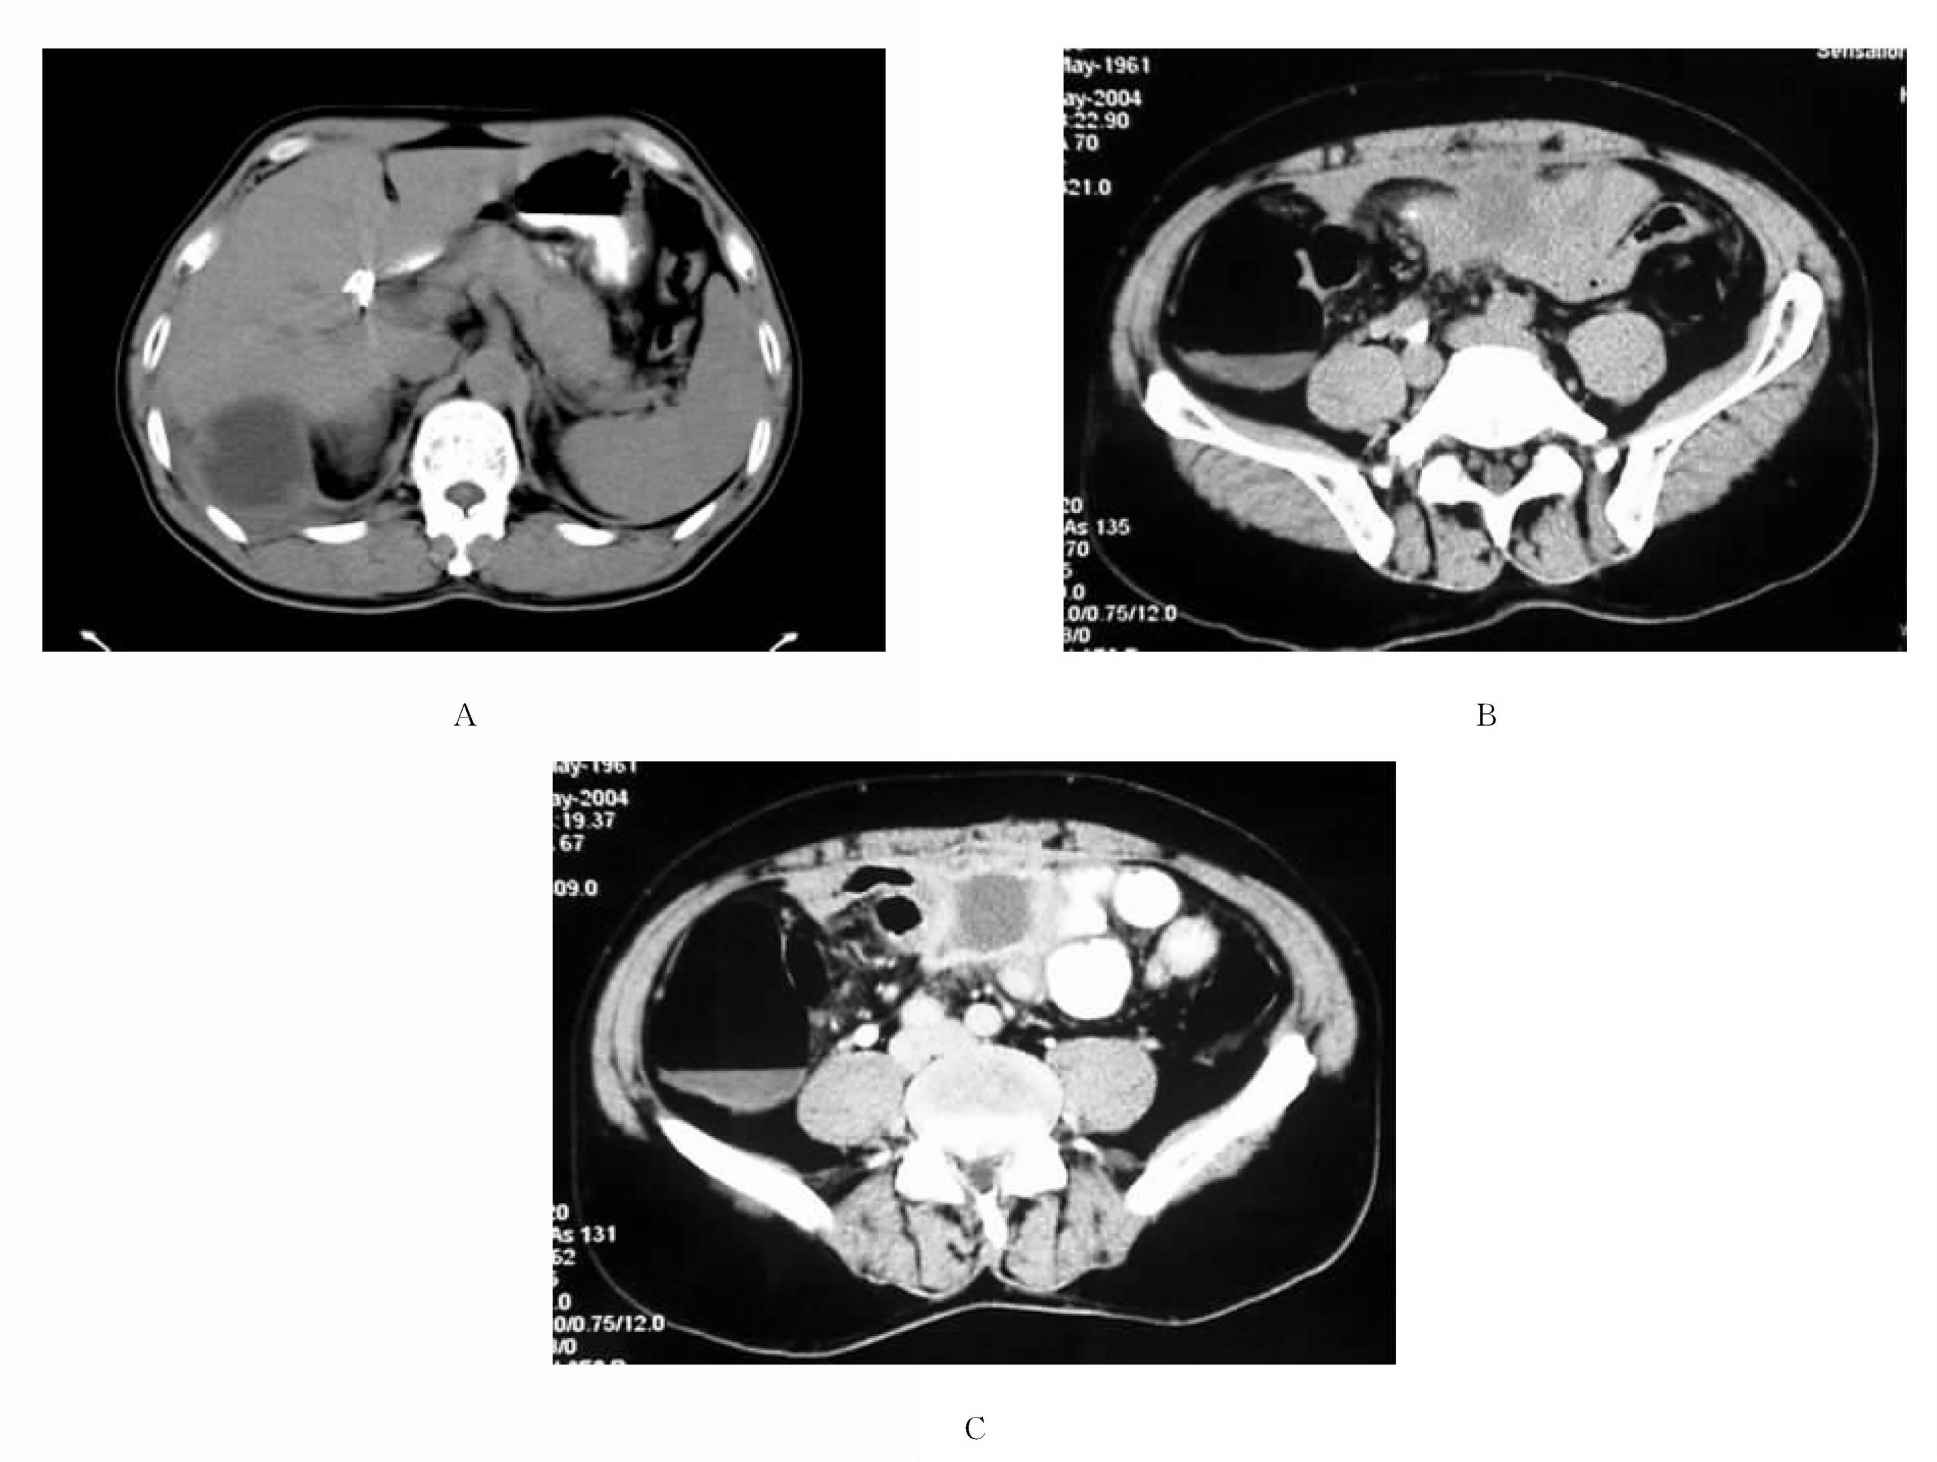
\includegraphics[width=.7\textwidth,height=\textheight,keepaspectratio]{./images/Image00373.jpg}
 \captionsetup{justification=centering}
 \caption{腹腔脓肿\\{\small A为膈下脓肿,右肝后方有厚壁水样密度灶;B、C为同一患者,是系膜间脓肿,分别为平扫和增强扫描,脓肿壁强化显著}}
 \label{fig18-4}
  \end{figure} 

\textbf{【鉴别诊断】}
需与肿瘤坏死液化、囊肿继发感染、包裹性腹腔积液、未能充盈造影剂的肠管等区别。腹腔脓肿与肿瘤、结核有着许多共性的CT表现,我们认为结合病史、临床症状和体征以及实验室检查WBC升高等是鉴别诊断的关键。

\subsection{腹膜炎}

腹膜炎大体可分为急性与慢性、弥漫性与局限性、继发性与原发性几类。病理上可为化脓性、癌性、乳糜性和结核性(后述)等。

\subsubsection{急性弥漫性腹膜炎}

\textbf{【病因病理】}
本病比较常见。多数继发于胃肠道穿孔(包括阑尾炎、憩室炎穿孔),胆道(主要指胆囊、胆总管等)结石、梗阻、感染、穿孔以及腹部术后并发感染等。病理表现主要包括腹膜炎症增厚、粘连,腹腔积液、积气,肠壁因纤维蛋白附着而增厚,以及肠郁张等。

\textbf{【临床表现】}
一般表现为腹痛、发热、全腹肌张力增强,有压痛及反跳痛,白细胞升高及核左移等。依病因不同可有一定差异。

\textbf{【CT表现】}
典型表现为:①腹腔积液、积气:但当无腹腔积气征象存在时,应注意与非炎症性腹腔积液相鉴别;②腹膜增厚、粘连:腹膜增厚通常比较均匀、普遍,壁层腹膜厚>2mm为增厚;粘连发生于腹壁与肠壁之间、肠与肠之间;③肠壁增厚、肠郁张甚至继发粘连性肠梗阻征象;④还可继发胸部改变如胸腔积液、肺底炎症、亚段肺不张等。

\subsubsection{局限性腹膜炎}

\textbf{【病因病理】}
常发生于脏器炎症致局部腹膜受累(例如急性阑尾炎穿孔并右下腹局限性腹膜炎),也可发生于弥漫性腹膜炎的局限化。其病理表现与弥漫性腹膜炎相似。

\textbf{【临床表现】}
也有腹痛、发热,白细胞升高及核左移等。但腹肌张力增强、压痛及反跳痛为局限性。

\textbf{【CT表现】}
与弥漫性腹膜炎相似。①腹膜增厚;②腹腔积液;③腹壁水肿;④脏壁增厚及粘连;⑤肠郁张(肠充气、扩张)等征象。上述征象局限于某一区域。此外,还可能显示一定的原发灶征象例如阑尾增粗、结石、周围粘连、软组织肿块等(图\ref{fig18-5})。

\begin{figure}[!htbp]
 \centering
 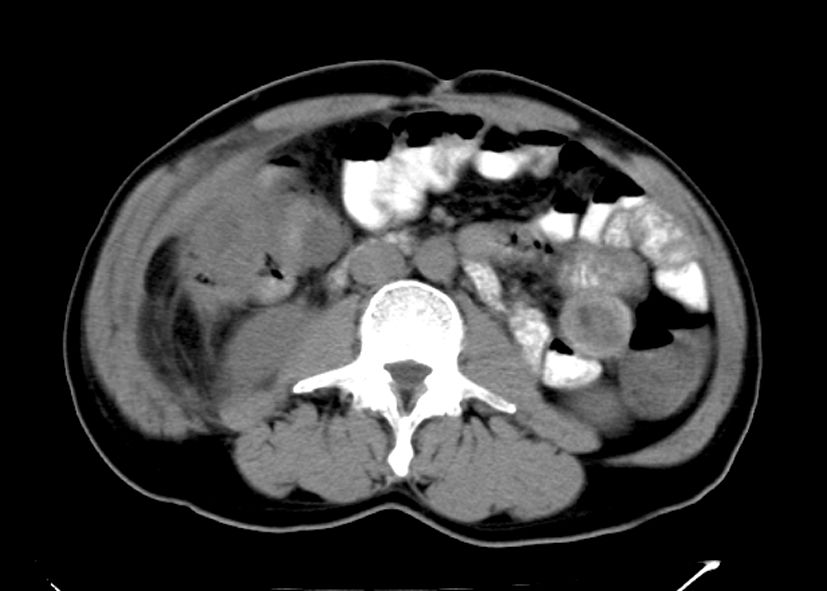
\includegraphics[width=.7\textwidth,height=\textheight,keepaspectratio]{./images/Image00374.jpg}
 \captionsetup{justification=centering}
 \caption{腹膜腔炎块\\{\small 右中腹部有软组织肿块,边缘毛糙、界限不清晰}}
 \label{fig18-5}
  \end{figure} 

国内有学者认为:所有急腹症病例,病灶邻近之网膜、系膜血管增粗、密度增高或表现为多数条索状、网格状影,可能与充血水肿、炎性浸润有关。网膜肿瘤周围变化远不及急性炎症病变周围显著,但常鉴别困难。

\subsubsection{原发性腹膜炎}

\textbf{【病因】}
主要有两种来源:①败血症在腹部的表现;②女性病例,尤其是年龄较小的女性病例,细菌可从阴道经子宫、输卵管逆行进入腹腔。此外,肝硬化、肾炎以及心肾功能衰竭伴腹水者患病率高,还与系统性红斑狼疮、肉瘤样病变、卵巢膜细胞瘤有关。

\textbf{【CT表现】}
除一般无腹腔积气表现征象外,其余所见基本同急性弥漫性腹膜炎。

\subsection{结核性腹膜炎}

本病是由结核杆菌引起的腹膜炎症,发病率仅次于肺结核及肠结核。

\textbf{【感染途径】}
有两条:①腹腔病灶如肠结核、肠系膜淋巴结结核或盆腔结核活动灶直接蔓延到腹膜;②血行感染:如粟粒性肺结核、肺原发综合征等血行播散至腹膜所致,肺结核患者3.5%发生腹膜结核。

\textbf{【病理】}
分为3型:①粘连型;②腹水型;③干酪型。各型的腹膜表面均可见粟粒结节,腹膜广泛粘连、网膜增厚、纤维增生收缩成团。腹水型较多见,为渗出液。干酪型少见,以干酪坏死为主,腹腔内见局限性积液或脓肿,干酪灶可侵及肠管形成内瘘。

\textbf{【临床表现】}
本病多起病缓慢。全身症状主要为中度发热、食欲不振、乏力、盗汗和体重下降等,脐周、上腹或全腹不适或钝痛。多数腹部有“揉面感”体征,可触及包块;腹水型者有腹水体征。常继发肠结核、结核性输卵管炎或肠系膜淋巴结核。

\textbf{【CT表现】}

1.腹腔内不规则软组织肿块:由干酪灶、纤维化肿块和粘连的肠曲包绕而成,密度不均,少有强化。有时呈囊实样肿块,亦可坏死液化灶与肠管沟通形成边界模糊的肿块,内可见液气平面。

2.肠系膜淋巴结增大:分散或融合成分叶状肿块,增强扫描多呈环状或多个环状强化有一定特征。

3.高密度腹水:CT值多为25~35Hu,腹水分布弥散或局限。

4.小肠曲粘连、位置固定或分布不规则,可有轻度到中度肠管扩张。

5.腹膜增厚表现:①粟粒状病灶:即腹膜上小米粒大小的结节,周围有程度不同的渗出和增殖。CT表现为“污迹”腹膜,增强扫描无强化。②腹膜结节:以结核性肉芽肿为其病理特点。CT表现为腹膜上软组织样结节,增强扫描可明显强化。③饼状网膜:病理成分以纤维组织和干酪坏死为主,多伴有肠粘连。CT表现为网膜扁块状增厚,边缘较清,表面明显凹凸不平,增强扫描有不同程度的强化。

\textbf{【鉴别诊断】}

1.腹膜腔肿瘤、炎症、结核有着许多共性的CT表现,均可出现腹腔肿块、腹水、肠粘连、淋巴结肿大,结合临床综合诊断甚为重要。

2.国外有学者认为与癌性腹膜增厚的鉴别主要观察壁层腹膜。轻度而光滑的增厚,提示为结核性;结节状不规则增厚提示为癌性。单从结核性腹膜炎的CT征象而言,“污迹”腹膜最为常见。

\subsection{肠系膜脂膜炎}

本病又称腹内脂膜炎。系一种以慢性炎症为主的肠系膜性疾病,以纤维化为主者称为缩窄性或回缩性肠系膜炎。

\textbf{【病因】}
不十分明确,大多为原因不明的特发性,部分与外伤(包括手术)、感染(但除外胰腺炎)、溃疡病、局部缺血有关。还有报道30%与恶性肿瘤(其中50%为淋巴瘤,还有白血病、骨髓瘤、胸膜间皮瘤等)有关;另有报道是自身免疫性疾病,与特发性腹膜后纤维化、多发性软骨炎、系统性红斑狼疮等有关。

\textbf{【病理】}
主要为肠系膜增厚,常局限于肠系膜根部,亦可延及到肠管边缘,乙状结肠系膜亦可侵犯。纤维化为主时肠系膜收缩呈团块状,质地坚硬或呈橡胶状,直径1~15cm。有报道肠系膜根部单发结节60%,多发结节15%和广泛系膜增厚20%。切面呈黄色或棕黄色,灰色斑块代表脂肪坏死。组织学上病变由坏死、退变的脂肪组织,以及嗜脂细胞、淋巴细胞、浆细胞、嗜酸性细胞和不同程度的纤维组织组成,可见钙化。淋巴管受阻可致肠黏膜下淋巴管扩张,并致肠狭窄、乳糜胸水和腹水。本病最终形成纤维瘢痕。

\textbf{【临床表现】}
发病年龄为20~80岁,60~70岁为高峰,男女发病比例为(1.5~1.8)∶1。一般表现为发热(中低度发热)、痉挛性腹痛、恶心、呕吐、厌食、体重下降、恶液质、腹泻、便秘、便血。50%可扪及压痛性肿块,一般无腹膜刺激征和腹水。实验室检查部分有WBC升高、ESR增快,贫血、低蛋白血症和C反应蛋白(CRP)升高。本病有自限性。

\textbf{【CT表现】}
典型表现为围绕系膜大血管(不受累及)、边界清楚、密度不均的单个或多个软组织密度肿块,其内可见脂肪密度或低密度囊变区。大血管和肿块周围见“脂肪晕征”,肠袢向四周移位。部分表现为系膜根部围绕系膜血管的单个或多个以脂肪成分为主的肿块,内有散在放射状索条样、结节样(多小于5mm)软组织密度区。有的表现为有包膜的密度不均匀肿块,内有脂肪、水样或软组织密度区。少数表现为多房囊性肿块(由于淋巴管阻塞引起的淋巴管扩张)。此外上述各种表现形式的病灶,中心均可见钙化。

总之,本病以脂肪晕征(或脂肪环征)、肿瘤样囊变和软组织结节为特征。本病与类癌、脂肪类肿瘤CT表现难以鉴别,且在诊断时应除外胰腺炎、肠道感染等疾病引起的脂肪坏死。

\subsection{腹茧症}

本病是临床外科非常罕见的腹部疾病。

\textbf{【病因病理】}
尚不明确,有以下几个方面:①性别和地区:多发生于热带和亚热带地区,且女性多发,可能由于病原体经女性生殖道逆行感染引起亚急性腹膜炎的后遗症。②药物因素:长期应用β受体阻滞剂,导致胶原的过度增生所致。③原发性腹膜炎:肝硬化、肾炎以及心肾功能衰竭伴腹水者患病率高,此外与系统性红斑狼疮、肉瘤样病变、卵巢膜细胞瘤有关。④医源性:长期不卧床的腹膜透析患者;腹腔-静脉、脑室-静脉引流术的腹腔滞留导管可引起硬化性腹膜炎。

其病理特征是小肠部分或全部被一层灰白色、致密且质地坚硬的纤维结缔组织膜包裹,形似蚕茧故名腹茧症,又称特发性致死性腹膜炎。有人认为它是硬化性包裹性腹膜炎的一种特殊类型。

\textbf{【临床表现】}
好发于青年女性。表现为不明原因的不完全性机械性肠梗阻,有腹痛、呕吐,但缺乏典型肠梗阻的4大症状。腹部可触及质地较软的包块。

\textbf{【影像学表现】}

1.CT特点为扩张的小肠袢固定腹部某一部位,被增厚的纤维腹膜所包裹或分隔呈串珠状,肠系膜挛缩。

2.小肠钡剂造影显示全部或部分小肠积聚在某一部位,不易分离,钡剂在小肠通过的时间明显迟滞。

\textbf{【鉴别诊断】}
本病应注意与腹膜包裹症相鉴别。后者也罕见,属先天发育异常,为小肠被相对正常的腹膜结构包绕,是胚胎发育中脐囊的残留,该囊随小肠的发育坠入腹中,并包绕小肠,颈部位于十二指肠,故又称“十二指肠旁疝”。该层腹膜为正常腹膜结构,与小肠无粘连,不影响肠蠕动,不易产生肠梗阻,有别于腹茧症。两者CT表现类似,不易鉴别,但腹茧症多发于热带和亚热带地区,且女性多见。

\subsection{网膜扭转}

\textbf{【病因病理】}
本病分为原发性和继发性两种类型。发生扭转的前提可能是网膜肥厚畸形、动力增加或网膜存在特异性炎症,突然咳嗽、体位改变、提取重物、外伤、饱食、剧烈运动等为诱发因素。继发性者与网膜粘连、疝、囊肿或肿瘤有关。扭转发生后其远侧出现淤血,甚至梗塞坏死。

\textbf{【临床表现】}
男女发病相近。进行性腹痛为主要症状,最后疼痛常局限于右下腹,半数伴恶心及发热,病程平均48h。局部有腹膜刺激征,半数患者外周血中WBC升高。与阑尾炎或胆囊炎很相似。

\textbf{【CT表现】}
腹腔内脂肪密度肿块,特征性的CT征象是含有纤维索条和脂肪的网膜褶襞向“肿块”(扭转处)呈放射状汇集,类似小肠扭转时系膜的改变。

\textbf{【鉴别诊断】}
应考虑到血管平滑肌脂肪瘤、脂肪瘤、脂肪肉瘤、畸胎瘤和术后纱布存留。

\subsection{网膜原发性节段性梗塞}

本病罕见,系原因不明的网膜急性血管病变。

\textbf{【病因病理】}
本病变多见于网膜右侧,可能与网膜右侧脂肪多且活动度大有关;诱发因素有患者体位改变、饱餐后血管充血、腹腔压力突然增加等。多数梗塞灶直径6~8cm。镜下见病变区动、静脉血栓形成,早期出血性梗死伴脂肪坏死,随后炎性细胞浸润,最后被纤维组织取代。

\textbf{【临床表现】}
男多于女,任何年龄均可发病。较多见于肥胖者,表现为剧烈腹痛,75%发生于右下腹,活动时疼痛加剧,伴发热、腹膜刺激征,WBC升高。易误诊为阑尾炎或胆囊炎。

\textbf{【CT表现】}
病灶多位于网膜右侧,几乎均位于腹腔右前方,在脐水平或稍上方层面、右半结肠与腹壁之间见局限性的脂肪密度肿块。病灶大小3~15cm,呈椭圆形或饼状。肿块内可见散在高密度条状影。

其CT表现难与网膜转移瘤、脂肪肉瘤等鉴别,与网膜扭转也不能完全鉴别。

\subsection{小肠系膜病变}

1.小肠系膜根部病变

小肠系膜是将空、回肠连系于后腹壁的双层腹膜反褶,固定于后腹壁的部分称为小肠系膜根。与小肠系膜根相邻接的重要结构有肝十二指肠韧带、结肠系膜、胰头区神经丛及淋巴组织(见表\ref{tab18-1})。

\begin{table}[htbp]
\centering
\caption{肠系膜根病变}
\label{tab18-1}
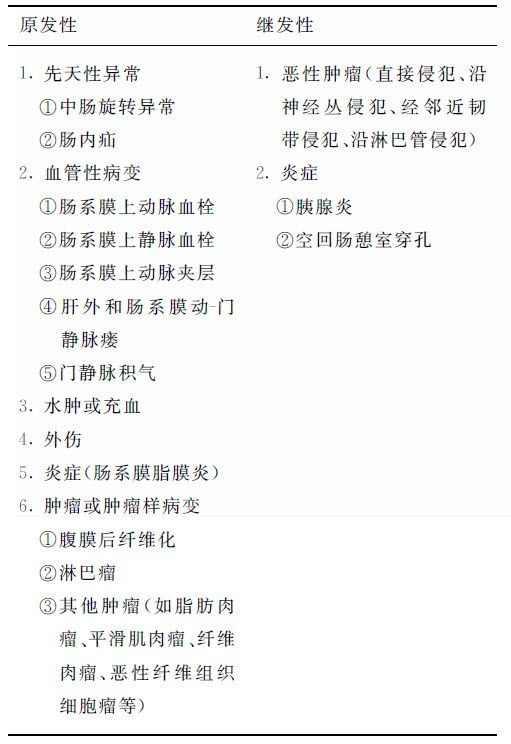
\includegraphics[width=\textwidth,height=\textheight,keepaspectratio]{./images/Image00375.jpg}
\end{table}

2.肠系膜混浊

肠系膜主要由脂肪及穿行于其中供应肠道的动静脉和淋巴管构成。肠系膜脂肪的密度改变常提示有肠系膜或肠道病变,故有作者以“肠系膜混浊”描述肠系膜脂肪受炎症细胞、液体(水、淋巴液和血液)、肿瘤浸润及纤维化的CT表现。

肠系膜脂肪的CT值类似于皮下及腹膜后脂肪(约-100~-160Hu),肠系膜血管常呈横行或显示其断面。当肠系膜混浊时,其脂肪CT值增加到-40~-60Hu,动、静脉失去锐利边缘。

3.肠系膜异常的相关征象和疾病

肠系膜异常的征象和疾病包括:①弥漫性肠系膜病变:包括水肿(图\ref{fig18-6})、淋巴水肿、出血、损伤及感染。②局灶性肠系膜肿块:如淋巴瘤等恶性肿瘤、肠系膜囊肿、纤维瘤、畸胎瘤、脂肪瘤及炎症等。③多发性肠系膜肿块:最常见为淋巴结增大如淋巴瘤、淋巴增殖紊乱、转移瘤、结核、猫抓病或真菌感染、淋巴结炎、结节病等。

\begin{figure}[!htbp]
 \centering
 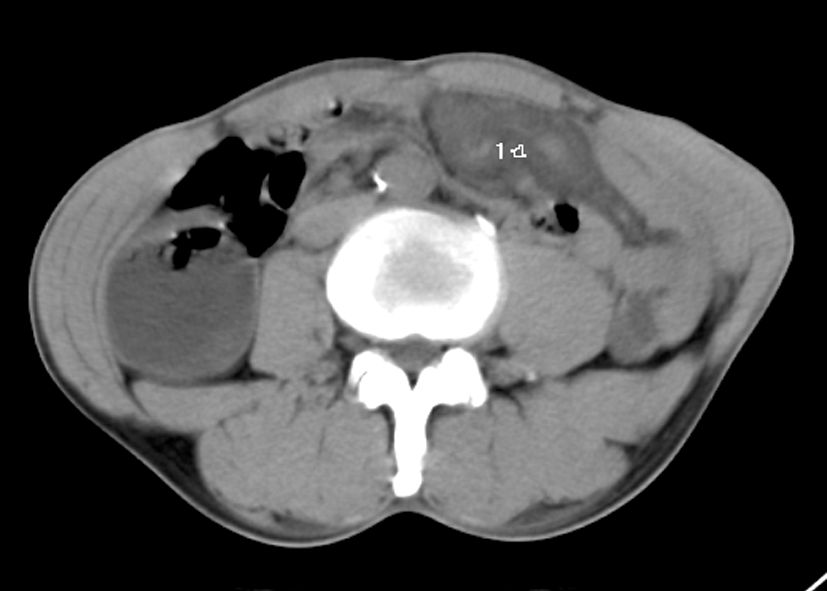
\includegraphics[width=.7\textwidth,height=\textheight,keepaspectratio]{./images/Image00376.jpg}
 \captionsetup{justification=centering}
 \caption{肠系膜水肿\\{\small 左侧小肠系膜呈大片状密度增高,近水样密度(腹部术后局部肠粘连、嵌顿所致)}}
 \label{fig18-6}
  \end{figure} 

\section{腹膜腔肿瘤}

\subsection{概述}

\subsubsection{腹膜的良、恶性肿瘤}

1.良性肿瘤:稍多见的是肠系膜硬纤维瘤,其他如脂肪瘤、纤维瘤、纤维组织细胞瘤、平滑肌瘤、血管瘤、神经源性肿瘤、淋巴管瘤、血管淋巴管样错构瘤、间叶瘤、乳头状囊腺瘤、脂肪母细胞瘤、淋巴管瘤、皮样囊肿、黏液囊肿等均极为少见。寄生虫性囊肿不属于真性肿瘤,偶发于腹膜。

2.恶性肿瘤:较多见,却很少原发,而以继发者多见。原发性常见为恶性间皮瘤,而脂肪肉瘤、平滑肌肉瘤、恶性间质瘤、神经纤维肉瘤、恶性纤维组织细胞瘤、血管外皮细胞肉瘤等少见,亦有腹膜腔成骨肉瘤的报道。

3.CT特点:在CT上常为单发、形态多变。一般囊性肿块(可有强化的壁结节和间隔)及均质实性肿块(如纤维瘤、神经纤维瘤及平滑肌瘤)强烈提示为良性;而囊实混合性强烈提示为恶性。边缘不清晰提示为恶性,边缘清晰对鉴别良恶性意义不大。

\subsubsection{腹腔脏器外囊性病变的分类}

该类病变是指腹膜腔内、腹膜后及肠系膜上的腹部脏器间隙内发生的以囊性为主的病变。常见的有以下4类:①先天或后天发育障碍性病变:如囊性淋巴管瘤、中肾管囊肿(主要发生于肾输尿管行程)、肠重复畸形;②肿瘤性病变:如囊性畸胎瘤(好发于腹膜后及盆腔)、囊性转移瘤;③外伤性病变:如慢性血肿;④感染性病变:如腹部脓肿。上述病变尤其囊肿类病变,应注意结合病史与胰腺炎性假性囊肿相鉴别。

\subsubsection{肠系膜肿块的位置诊断}

国外文献报道:凡腹腔肿块压迫胰腺、主动脉、腔静脉、肠管后移,而不侵及邻近器官,不能确定起源于哪个脏器,并能与腹膜后分开,周围被肠管完全或部分包绕,而肠管本身正常者;肿块附近肠系膜叶增厚,脂肪密度增高,血管增粗、模糊乃至消失(模糊肠系膜),肠系膜上动、静脉完全或部分被包绕(“三明治”征,该征是淋巴瘤的特征,但亦见于转移瘤)者,多提示或确诊为肠系膜肿瘤。

\subsection{肠系膜硬纤维瘤}

\textbf{【病理】}
本病起源于肠系膜纤维组织,其切面呈编织状,质硬、光滑、边界清楚。镜下由分化成熟的纤维组织构成,无包膜。

\textbf{【临床表现】}
肿瘤小时一般无症状。大者常因压迫、推移相邻脏器而产生相应症状,如腹胀、腹痛等。

\textbf{【CT表现】}
肿瘤呈边界清楚的软组织肿块,多数较大,密度可均匀,亦可中心坏死而出现低密度区。肿块周围见纤维组织增生形成的条状影,呈星芒状。邻近肠管被推移。

\textbf{【鉴别诊断】}
与其他良、恶性肿瘤常难以鉴别。①平滑肌类肿瘤:罕见,以回肠系膜多见。密度不均,边缘多较光滑,有不均匀强化。较大时可压迫推移邻近肠管,有时难以鉴别。②脂肪肉瘤:少见。密度不均,多呈混杂密度,即含脂肪密度、水和软组织密度,有的单呈软组织密度而鉴别困难。常因为是无痛性肿块而长得很大,并侵犯邻近结构。肿块有不同程度的强化。

\subsection{肠系膜囊肿}

\textbf{【病理】}
本病分为两类:①真性囊肿:其内衬覆上皮细胞,属先天性。又分为浆液性、乳糜性、表皮样囊肿。②假性囊肿:其内无上皮细胞衬覆,多由外伤性、感染性及肿瘤性病变所致。故有学者将肠系膜囊肿称为囊性淋巴管瘤是不合理的,囊性淋巴管瘤属肠系膜真性囊肿的范畴。

\textbf{【临床表现】}
可发生于任何年龄。囊肿小时可无症状。较大者可引起慢性腹痛。当囊肿发生破裂、扭转、感染、出血及压迫肠管等情况时,可表现为急腹症。有些可触及腹块,甚至腹围增大。可伴随恶心、呕吐、纳差等症状。

\textbf{【CT表现】}
囊肿发生于空、回肠系膜,亦可见于盲肠、横结肠和乙状结肠系膜内,以小肠系膜发生率最高。通常为单发,亦可多发。大小不一,从数厘米到充满整个腹腔的巨块状。囊肿呈圆形或椭圆形均质囊性肿块,CT值近似水或大于水,囊壁不强化。表皮样囊肿的CT值低于水。感染性囊肿壁厚,密度不均,可钙化,强化显著。

\subsection{肠系膜淋巴管瘤}

本病多见于小儿,是一种发育畸形。

\textbf{【病理】}
囊内衬覆内皮细胞,属真性囊肿。易侵犯小肠系膜。本病分为单纯性、海绵状、囊性3类,其中囊性多见,常有分房,体积较大。

\textbf{【临床表现】} 与上述肠系膜囊肿相似。

\textbf{【CT表现】}
囊型呈圆形或椭圆形、囊壁菲薄、界限清晰的均质水样密度肿块,可有分房。有时CT值较高,合并感染或出血者CT值可显著升高、密度不均匀。海绵状型呈软组织肿块,密度不均,CT值0~60Hu不等,界限清楚。

\textbf{【鉴别诊断】}
应与肠系膜淋巴血管瘤鉴别。后者即淋巴管瘤伴有增生的毛细血管,CT表现囊壁较薄、光滑,有较多粗大的小梁不全分隔呈网状,粗大的小梁强化著;因易出血可急剧增大,此时CT出现液-液平面。

\subsection{腹膜间皮瘤}

本病是源于腹膜上皮和间皮组织的恶性肿瘤,占所有间皮瘤的20%。

\textbf{【病因病理】}
病因与接触石棉有关。组织学分为上皮型(50%)、结缔组织型(25%)和混合型(25%)3类。胸腹腔可同时发病。病变倾向于沿腹膜表面扩散呈浸润性生长,淋巴和血行转移少见。

\textbf{【临床表现】}
好发于40~70岁男性。无特殊症状,如体重减轻、腹痛、消化不良、发热、恶心和腹水等。

\textbf{【CT表现】}
腹膜弥漫性不规则增厚,且密度升高,有的可见钙化,系膜间血管模糊。也可呈弥漫或局限的结节或肿块,尤以腹水衬托下的肝、脾边缘结节显示更清楚。网膜或系膜肿块呈薄的糕饼状,增强扫描强化程度不一,与继发性网膜肿块难以区别。囊性腹膜间皮瘤压迫肝缘呈扇形。肠系膜僵硬、收缩呈星形放射状。肠曲固定、集中,呈扇形分布。大网膜受累,见肠管与前腹壁间距增加,其间见不规则软组织肿块。腹水常见,量多少不等。

\subsection{腹膜转移瘤}

\textbf{【来源】}
继发性有4种来源:①原发癌瘤经系膜和韧带附着处直接向腹膜蔓延;②肿瘤已侵犯到脏器的浆膜面,癌细胞脱落而产生腹膜种植;③淋巴转移相当常见;④血行播散。

\textbf{【临床表现】}
有原发肿瘤的症状及恶性肿瘤的全身表现。还可有腹水、腹块,甚至肠梗阻的症状。

\textbf{【CT表现】}

1.腹水:是最常见的表现,其量多少不一。

2.壁层腹膜增厚:其厚度>2mm为增厚,呈结节状、宽带状或块状增厚。国内有学者报道以右侧腹壁多见,次为左侧腹壁和前腹壁。国内还有学者通过腹膜腔造影观察腹膜转移,并认为腹膜上任何大小的软组织结节、长度>10mm的斑块及短条状影均是腹膜转移瘤的表现。

3.大网膜及肠系膜改变:分为以下几类:①污垢状:表现为均匀脂肪密度的肠系膜或大网膜内出现多数细小的点状、短条状污垢样影(图\ref{fig18-7}A)。②结节状。③饼状大网膜:结肠或小肠与前腹壁之间呈现密度不均的饼状软组织影,但该征亦可见于结核。④肿块状:单个或多个(图\ref{fig18-7}B~D)。⑤混合型。

\begin{figure}[!htbp]
 \centering
 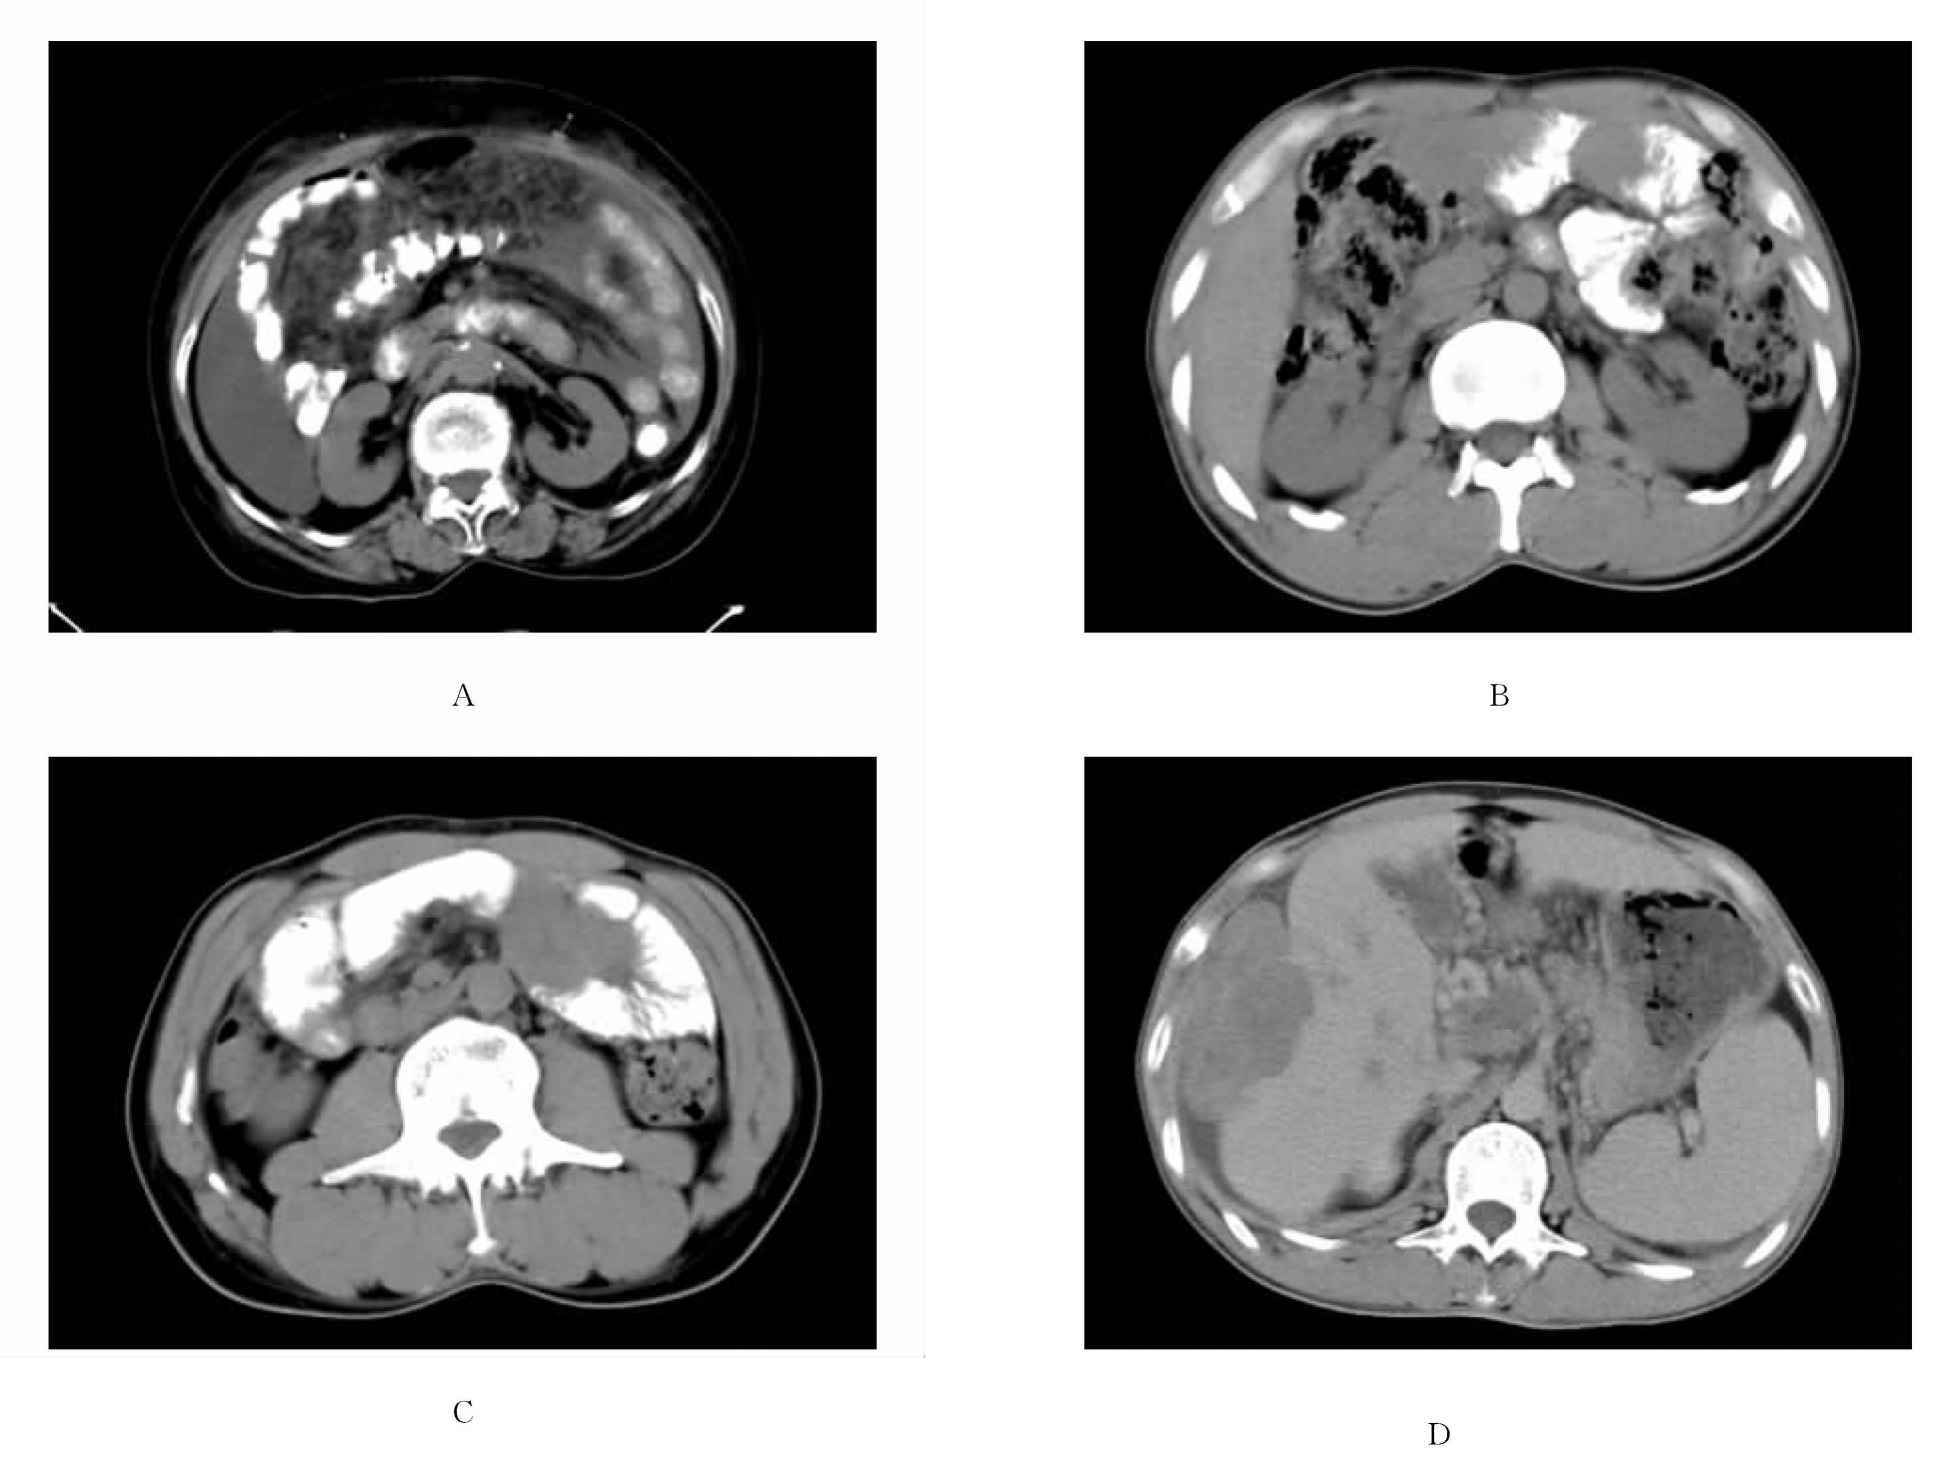
\includegraphics[width=.7\textwidth,height=\textheight,keepaspectratio]{./images/Image00377.jpg}
 \captionsetup{justification=centering}
 \caption{腹膜转移瘤\\{\small A、肠系膜和大网膜内出现许多细小的点状、短条状污垢样影;B、C为同一患者,来自胃癌转移;左侧小肠系膜区和大网膜区有软组织肿块。D为肝癌腹膜块状转移,肝脏边缘呈波浪状受压}}
 \label{fig18-7}
  \end{figure} 

4.腹腔内多囊性占位:如卵巢黏液性囊腺癌转移可见此征,亦可呈单囊状,包裹性腹水可以是其腹腔种植的惟一表现。

5.肠管壁增厚和肠管移位:主要由于脏层腹膜受累所致,并可继发肠梗阻。

\subsection{腹膜假性黏液瘤}

本病又称假性黏液瘤性腹水或假性腹水,系一种少见病,以腹膜腔内充以大量黏蛋白,形成假性腹水为特点。可分为良性、恶性和中间型。

\textbf{【病因病理】}
主要见于卵巢的黏液性囊腺瘤或囊腺癌及阑尾黏液囊肿,少见的来源还有卵巢畸胎瘤、卵巢纤维瘤、子宫癌、胃肠黏液腺癌、脐尿管癌、胆总管癌及肺癌。良性黏液囊肿破入腹腔是否会导致本病尚有争议。这种块状黏液是产生黏液的腺癌或囊肿破裂种植到腹膜,使腹膜间皮细胞发生变异而产生大量黏液。病理表现为纤维结缔组织中较大的黏液湖,可见少量上皮细胞增生;恶性病变中多见细胞排列紊乱和核分裂相。

\textbf{【临床表现】}
腹部渐胀大,一般情况可,病程可长达15年。可触及腹部包块,还可有食欲下降、消瘦等表现。有的表现为急腹症如肠梗阻、阑尾炎症状。几乎全部死于局部改变如肠梗阻。

\textbf{【CT表现】}
盆腔或下腹部见低密度肿块,呈多囊状,有明显的分房和厚度不一的囊壁;密度均匀,CT值近似水或略高(多>15Hu);边缘可见强化。有的病例边缘见斑点状、曲线状钙化,尤其在化疗、放疗后呈进行性钙化;慢性病例可见钙化的网膜饼。在上腹部包绕在肝脾周边造成波浪状或扇贝形压迹,与包裹性积液或局限性腹水相似。大量积液形似大量腹水,但肠管因粘连不能漂浮至前腹壁下即无飘浮感。肠系膜位置可见网状及分支状的脂肪间隙(且临床不易抽出腹水或呈血性黏液样物)。本病可继发感染发展为腹腔脓肿。

国外有学者认为,良性者病变“扇贝样”边缘大(>5mm),钙化多见;而恶性者大网膜明显增厚,形成网膜饼,“扇贝样”边缘相对小。

\textbf{【鉴别诊断】}
本病有时无特征性,与单纯腹水、腹膜炎、腹腔肿瘤不易区别。①腹水:腹膜假性黏液瘤一般有壁,其内有细小分隔,CT值较高,肠管受压多向中央聚拢移位;而腹水CT值多<10Hu,其内一般不见分隔,肠管呈向前的飘浮状等可予鉴别。②腹膜结核:腹部有揉面感,压痛,包块多为单个且较局限。

此外,还需与腹膜转移瘤、淋巴管瘤、畸胎瘤、胰腺囊肿及腹膜间皮瘤相鉴别。

\section{腹壁疾病}

\subsection{腹壁炎症}

\textbf{【病因】}
前腹壁内的炎症常由手术或外伤后伤口感染,或宿主防御机能低下(如糖尿病等),或腹内疾病如腹腔脓肿等蔓延所致。多数系产气菌感染所致。常侵犯皮下组织或肌层,亦可达整个腹壁。最严重的是坏死性筋膜炎,其发展迅速。

\textbf{【临床表现】}
局部红、肿、热、痛,若细菌毒力强可使炎症范围迅速扩大。

\textbf{【CT表现】}
弥漫性或局限性炎性肿胀常使腹壁增厚、边界不清,肌层间脂肪间隙模糊、消失。可伴散在性积液,CT值与水近似,脓液稠厚亦可高于水;范围可很广泛,如蔓延到腹膜后、阴囊和骨盆区(坏死性筋膜炎见后述)。当腹壁炎症局限形成脓肿时,见椭圆形或梭形软组织肿块。30%脓肿中央可见液性密度区,偶见液气平面。脓肿边界尚清,增强扫描其周边强化。脓肿可压迫邻近组织和脏器。腹腔内脓肿蔓延到腹壁可见相应表现。

\subsection{坏死性筋膜炎}

本病是一种少见、进展迅速的感染,其特征为皮下组织和筋膜广泛坏死,常伴严重的全身中毒症状,延误诊断和治疗不当常导致患者死亡。

\textbf{【病因病理】}
本病的高发人群是全身免疫机能低下及有小血管病变者,绝大多数为继发性,原因不明者仅占15%~18.2%,其中糖尿病是最常见的患病因素和危险因素,其他的相关因素甚多如酒精中毒、慢性肾功能衰竭、先天性白细胞减少、吸毒、肥胖、手术、化疗、放疗、使用免疫抑制剂治疗、脑血管意外、恶性肿瘤、急性感染性多神经炎、衰老、营养不良、滥用药物、痛风、艾滋病、梅毒、伤寒、周围血管疾病、尿外渗、阴茎异常勃起、过度性交、下泌尿生殖器或肛门旁软组织感染等。原发性或特发性以单种细菌感染为主,继发性者以多种细菌混合感染为主。病理上可见皮下小动脉栓塞、缺血,导致侵袭性感染发生。病变主要累及筋膜,无明显脓腔。

\textbf{【临床表现】}
本病病程急骤,个别可缓慢。男性多于女性,男女之比约为1.9∶1;可发生于任何年龄,以婴儿、儿童、老年人、免疫机能欠佳者发病率和死亡率高。可累及全身各部位软组织,以腹部、会阴生殖器、臀部、四肢为多,头颈部、胸部少见。早期表现为突发性疼痛、皮肤发红(12小时内)、皮肤水肿、软组织肿胀(24小时内)、发热,WBC升高;进展期皮肤弥漫性肿胀、红斑、水泡形成、皮肤坏疽,全身症状包括脓毒休克、多器官衰竭等。当组织坏死发生时,疼痛可进展直到感觉丧失。在原坏死性筋膜炎部位可再发感染。

\textbf{【影像学表现】}

1.平片表现:可显示软组织肿胀、增厚和纵隔、腹膜后及其他软组织内气体影,胸腔积液等。

2.CT表现:其CT征象为(图\ref{fig18-8}):①皮肤下弥漫性水肿增厚;②皮下脂肪条索状、网状强化;③筋膜增厚和(或)强化为其特征性改变;④软组织积气影,广泛积气是本病的标志,也可未见积气;⑤局部积液积脓、胸水、腹水;⑥肌肉不对称强化;⑦对比剂外渗,受累动脉或静脉坏死破裂所致;⑧颈内静脉或其他深静脉血栓或脓毒栓子;⑨淋巴结反应性肿大;⑩异物存留;⑪皮肤黏膜瘘;⑫随访CT最常显示的改变为持久筋膜强化、颈纵隔脓肿形成、进展性肌坏死等。

\begin{figure}[!htbp]
 \centering
 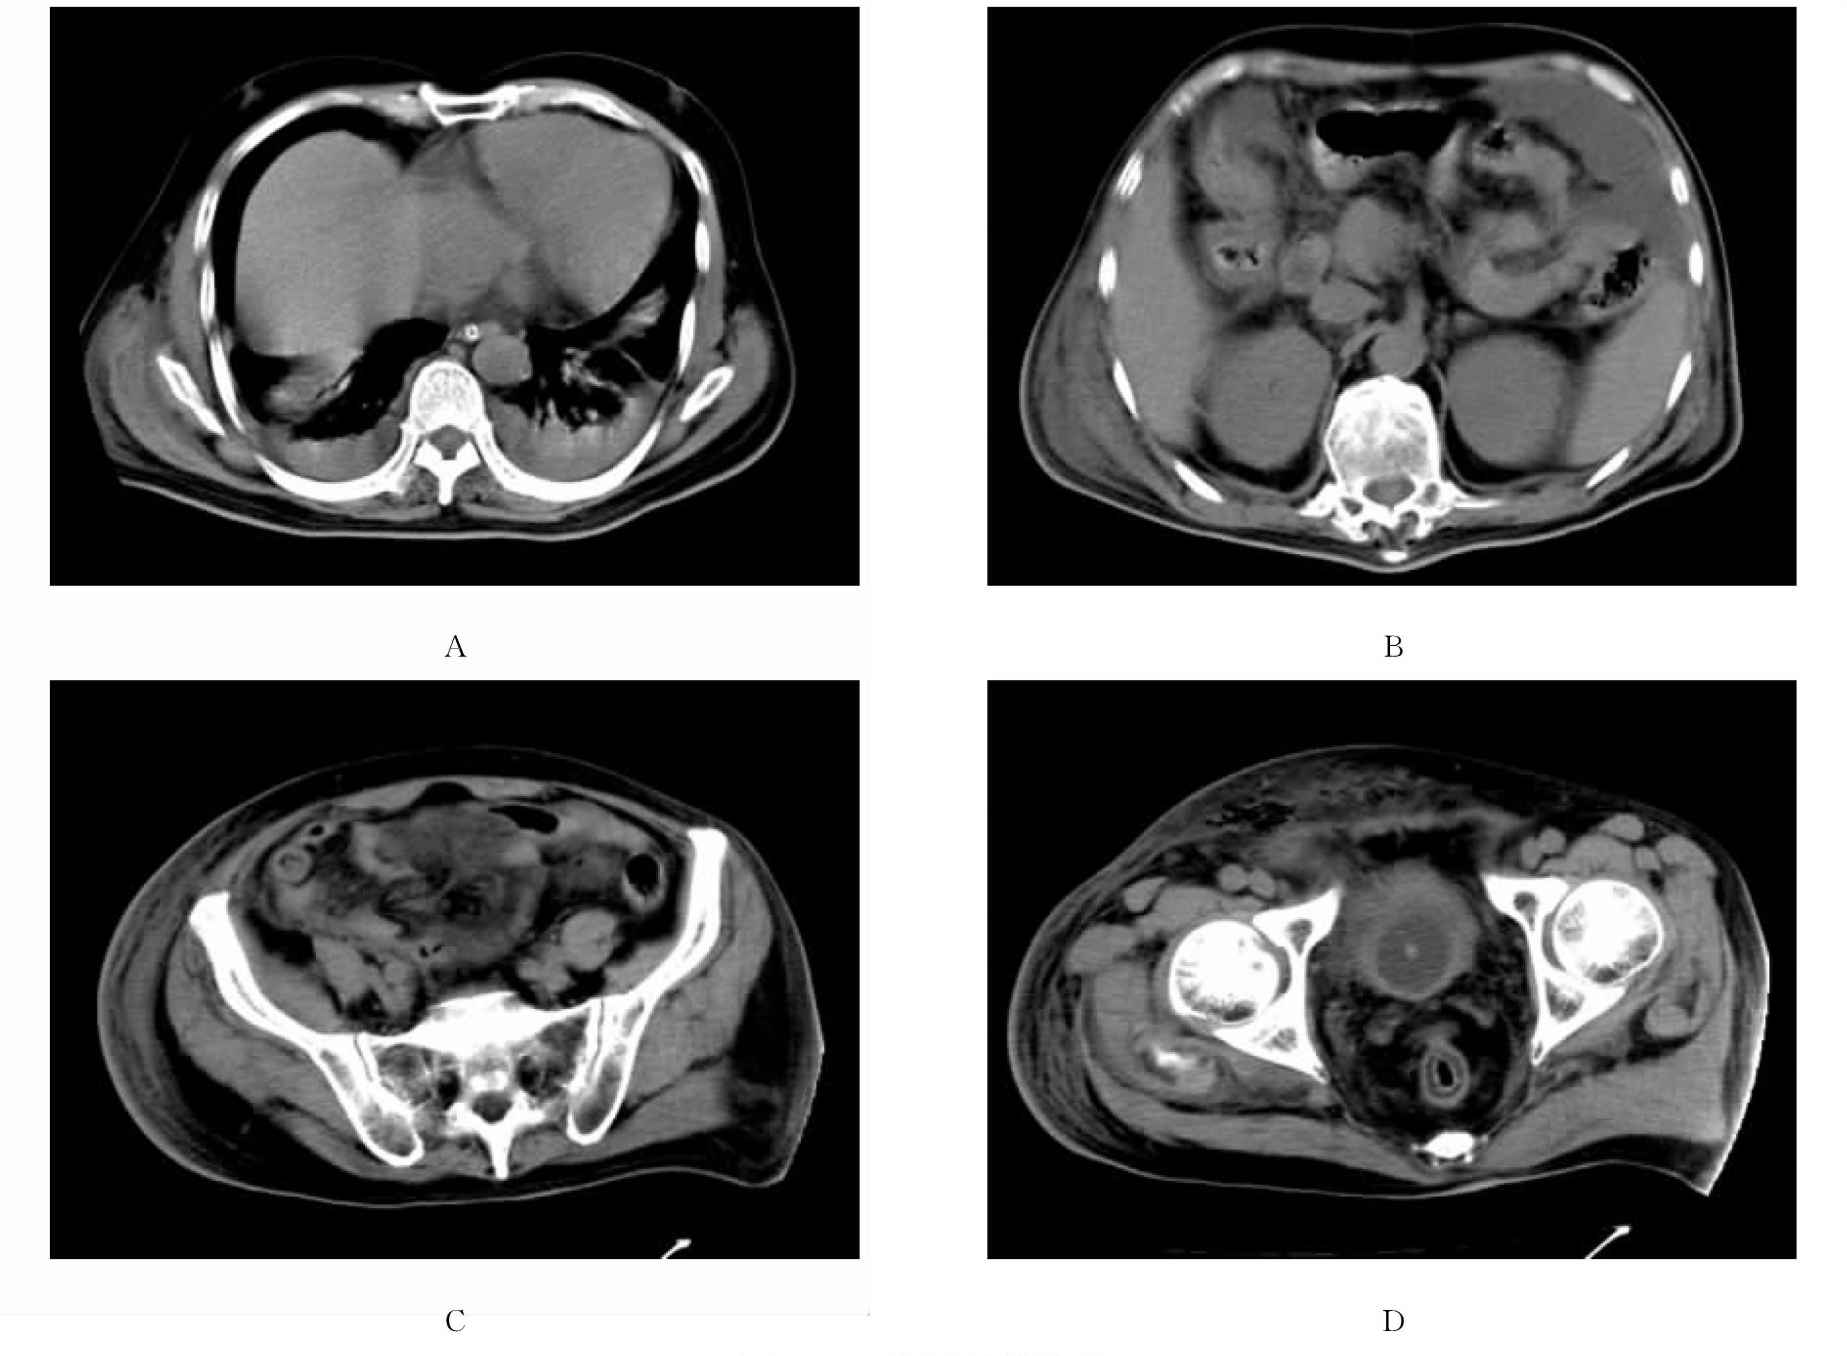
\includegraphics[width=.7\textwidth,height=\textheight,keepaspectratio]{./images/Image00378.jpg}
 \captionsetup{justification=centering}
 \caption{坏死性筋膜炎\\{\small A~D为同一患者,可见右侧腹壁皮下弥漫性水肿增厚、肌肉密度减低,前下腹壁也明显受累,左侧腹壁局限且轻度受累;双侧胸腔积液(A图);左侧前腹壁下和右侧腹壁下区域局限性腹腔积液(B图,以左侧显著)}}
 \label{fig18-8}
  \end{figure} 

此外,MR检查亦可明确显示皮下组织、浅深筋膜增厚,坏死组织、炎症或水肿等。

\subsection{腹壁积液}

腹壁积液罕见。

\textbf{【病因】}
一般见于长期家庭腹膜透析患者,透析导管处腹膜缺损,透析液漏入腹前壁皮下组织内。亦可见于切口疝患者腹水进入腹壁,向下可达阴囊。还可见于PTC后胆汁漏或腹腔穿刺后腹壁液体积聚。

\textbf{【CT表现】}
常呈梭形,其边缘尚光整;腹壁内的液体亦倾向于沿特定的解剖间隙扩散。如脐旁筋膜将下腹部腹膜外脂肪层分隔成膀胱前间隙和膀胱周围间隙,膀胱前间隙与腹壁腹膜前间隙相通,易于出现积液。

\subsection{腹壁血肿}

\textbf{【病因】}
一般继发于外伤、手术后和抗凝治疗后,偶为自发性。多累及腹直肌鞘。

\textbf{【临床表现】}
腹壁游离的血液可刺激腹膜产生剧痛,局部可触及肿块、皮肤变色。

\textbf{【CT表现】}
腹壁内见梭形或椭圆形肿块。急性期血红蛋白含量高,故密度高于或等于腹壁肌肉。随时间推移,血红蛋白分解吸收,故密度减低。血肿边缘清晰,晚期可见钙化。有时,陈旧性血肿因有形成分与血清分离沉淀,可见液平面。如果血肿内见散在小气泡、边缘不清晰,提示合并感染可能。

\subsection{腹壁疝}

腹腔内脏器或组织经腹壁薄弱点或缺损区向体表突出时可形成腹壁疝,典型者由疝环、疝囊、疝内容物或外被盖物等组成。

1.腹股沟疝

①斜疝:疝囊颈从腹壁下动脉之外侧的腹股沟管内环突出,疝入阴囊或女性大阴唇。②直疝:位于腹壁下动脉的内侧,常见于年老体弱者,疝囊颈宽大,不伸入阴囊,极少嵌顿。

\textbf{【CT表现】}
腹股沟区有突出在腹壁外的软组织块,边缘光整,似囊袋状,其密度与疝内容物有关(图\ref{fig18-9})。

\begin{figure}[!htbp]
 \centering
 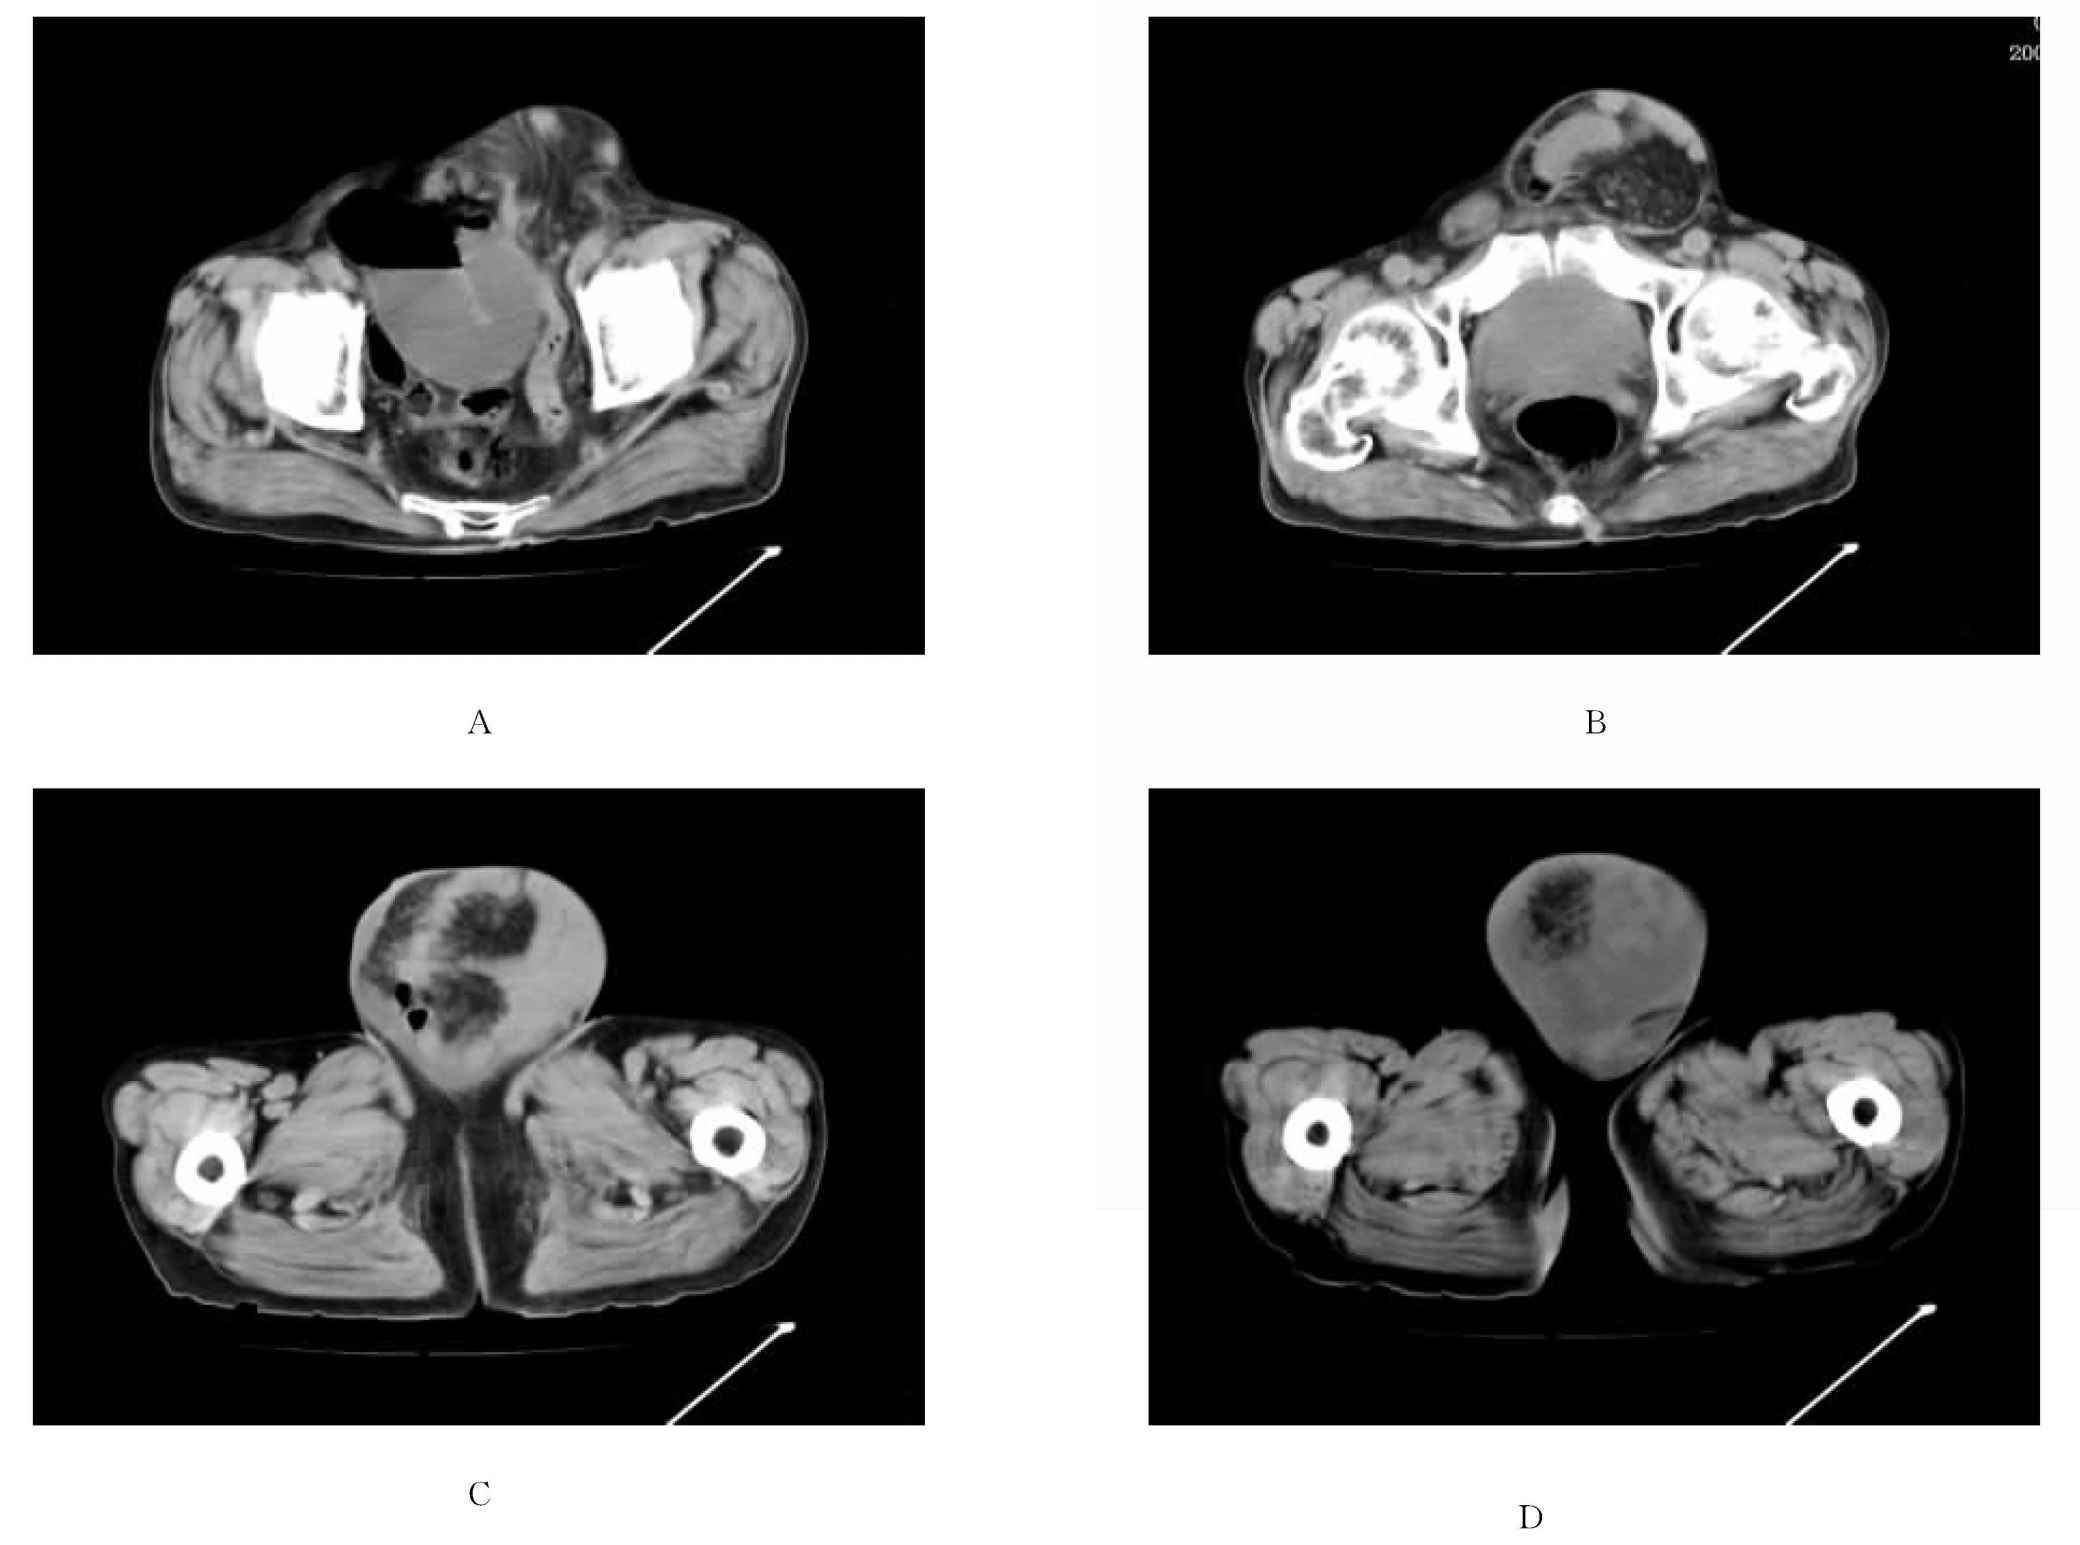
\includegraphics[width=.7\textwidth,height=\textheight,keepaspectratio]{./images/Image00379.jpg}
 \captionsetup{justification=centering}
 \caption{左侧腹股沟斜疝(伴有小肠嵌顿)\\{\small A~D为同一患者,左侧腹股沟区有突出在腹壁外至阴囊的软组织块,边缘光整;其内有含脂肪的腹膜和密度不一的肠管;近端肠管扩张}}
 \label{fig18-9}
  \end{figure} 

2.股疝

疝囊经股环、股管向股部卵圆窝突出的疝。中年以上妇女多见。

\textbf{【CT表现】}
疝囊位于耻骨结节的下外方,而腹股沟疝位于耻骨结节的上内方。

3.半月线疝

其发生率不到2%,但一旦形成并发嵌顿和肠绞窄的危险性高。

\textbf{【CT表现】}
疝囊经半月线突出,疝出物如仅为脂肪密度易误诊为脂肪瘤,但仔细分析可发现半月线处腹膜缺损。

4.切口疝

常见于腹壁纵形切口,多发生于术后4个月内,因为此间是腹壁已横断的肌肉、筋膜愈合的关键时期。

\textbf{【CT表现】} 原切口处腹膜缺损,疝本身表现无特殊性(图\ref{fig18-10})。

\begin{figure}[!htbp]
 \centering
 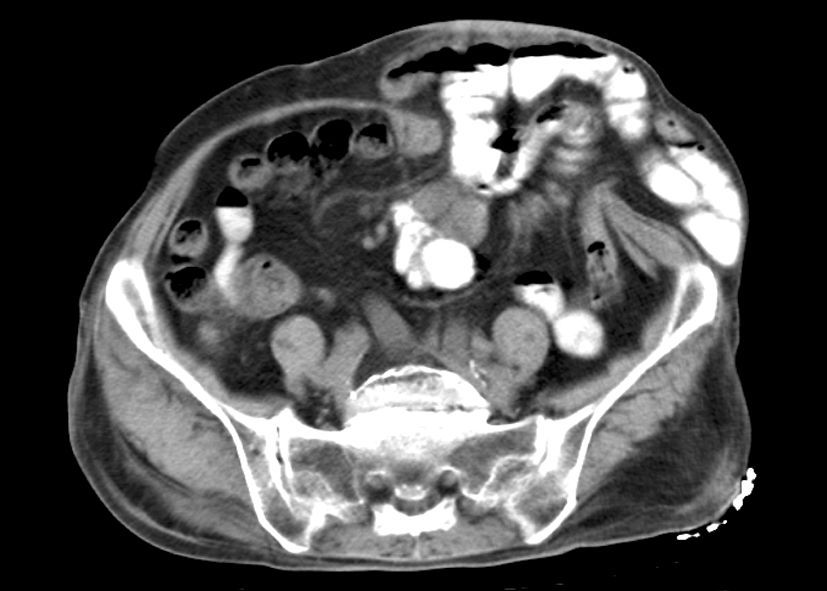
\includegraphics[width=.7\textwidth,height=\textheight,keepaspectratio]{./images/Image00380.jpg}
 \captionsetup{justification=centering}
 \caption{切口疝\\{\small 结肠癌术后,左侧前下腹壁有大量肠管和腹膜组织疝出}}
 \label{fig18-10}
  \end{figure} 

5.腰疝

发生于胁腹部。分为术后疝(如髂骨翼缺损疝)、上腰疝和下腰疝,后两者可为特发性,也可继发于外伤。

\textbf{【CT表现】} 可清楚显示疝内容物及邻近结构的解剖关系。

6.闭孔疝

发病率很低,是通过骨盆侧壁闭孔管向股部突出的隐匿性腹外疝,大多见于老年较瘦的妇女,这与女性骨盆宽阔和该处组织萎缩有关,由于左侧有乙状结肠掩盖,故多见于右侧。突出的疝块压迫闭孔神经产生大腿内侧和膝部放射性疼痛。

\textbf{【CT表现】}
主要表现有小肠梗阻,空回肠肠管扩张、积液;在闭孔外肌和耻骨肌之间可见疝囊;闭孔疝绞窄时,可见肠壁水肿增厚,增强扫描强化减弱;腹腔可见积液。

此外,常见的还有脐疝、白线疝等,临床易于诊断,CT能很好地显示。

\subsection{腹壁硬纤维瘤}

腹壁良性肿瘤以硬纤维瘤较常见,较少见的有脂肪瘤、血管瘤、上皮瘤、乳头状瘤、神经纤维瘤及皮样囊肿等。

\textbf{【病因病理】}
腹壁硬纤维瘤以脐下发生为主,一般认为与怀孕或分娩时肌肉紧张或鞘膜损伤有关。多发生在腹直肌鞘或腹外斜肌腱膜中。肿块由分化成熟的纤维组织构成,无包膜,可向周围肌肉组织浸润,与纤维肉瘤相仿但不发生转移,却有明显的术后复发倾向。

从上述病理表现可见应属于侵袭性纤维瘤病(或称瘤样纤维组织增生)的范畴,而纤维瘤(包括软纤维瘤和硬纤维瘤)应该有包膜、无侵袭性(详见二十二章第六节),故似乎一概称为腹壁硬纤维瘤不太确切。应将有包膜者(无侵袭性)称为腹壁硬纤维瘤;无包膜且有侵袭性者归为侵袭性纤维瘤病。对此有待进一步统一认识。

\textbf{【临床表现】}
腹壁硬纤维瘤80%见于女性,年龄20~40岁。多因局部触及肿块而就诊,一般无明显不适。

\textbf{【CT表现】}
常表现为结节状或块状软组织影,密度尚均匀,边缘光滑或模糊,附近结构受推移,局部腹壁隆起。但与腹壁恶性肿瘤可难以鉴别。

\subsection{腹壁恶性肿瘤}

\textbf{【病因】}
本病多为继发性的,亦有少数为原发性的。原发性以肉瘤为主,其中以横纹肌肉瘤、纤维肉瘤和平滑肌肉瘤最常见。继发性癌其转移途经有:①腹内癌沿淋巴管和淋巴间隙蔓延或直接侵犯,常见的原发灶有肝癌、胆囊癌和结肠癌等。②腹内癌瘤腹膜种植或血行转移到腹壁,或为其他组织结构转移再侵及腹壁,如大网膜转移瘤形成“网膜饼”后再浸润腹壁。

\textbf{【CT表现】}
①原发性者肿瘤多较大,直径常在5~15cm。其内密度不均,可见坏死的囊样低密度灶,亦可见高密度出血灶。边界不清,邻近结构受压或遭破坏。②转移性者可见腹内脏器肿块直接浸润破坏邻近腹壁,有时可见皮下转移结节。总之,转移性肿瘤如同时见到原发灶,确诊一般不难,必要时穿刺活检确诊。

\protect\hypertarget{text00026.html}{}{}

